\documentclass[a4paper,UKenglish,cleveref, autoref, thm-restate]{lipics-v2019}


\usepackage[utf8]{inputenc}
\usepackage{xspace}
\usepackage{url}
\usepackage{graphicx,graphics} 
\usepackage{color}
\usepackage{amsmath}
\usepackage{amsfonts}
\usepackage{amssymb}
\usepackage{amsthm}
\usepackage{algorithm}
\usepackage{algorithmic}
\usepackage{longtable}
\usepackage{complexity}
\usepackage{tkz-graph}
\usepackage{float}
\usepackage{tabularx} 
\usepackage{tkz-graph}
\usepackage{complexity}
 
%\renewcommand{\algorithmicrequire}{\textbf{Input:}}
%\renewcommand{\algorithmicensure}{\textbf{Output:}}

 
%\newtheorem{fact}{Fact}

\newcommand\pma{\textsc{pma}\xspace}
\newcommand\firstfit{\texttt{First Fit}\xspace}
\newcommand\compactpair{\texttt{Compact Pairs}\xspace}
\newcommand\metaoffset{\texttt{Meta Offset}\xspace}
\newcommand\greedyuniform{\texttt{Greedy Uniform}\xspace}
\newcommand\swapandmove{\texttt{Swap and Move}\xspace}
\newcommand\compactfit{\texttt{Compact Fit}\xspace}
\newcommand\greedypotential{\texttt{Greedy Potential}\xspace}
\newcommand{\todo}[1]{{\color{red} TODO: {#1}}}

\bibliographystyle{plainurl}% the mandatory bibstyle

\title{Scheduling Periodic Messages on a Shared Link} %TODO Please add
%\titlerunning{Dummy short title} %TODO optional, please use if title is longer than one line

%\author{Ma\"el Guiraud}{David Laboratory, UVSQ, France \and Nokia Bell Labs, France}{mael.guiraud@uvsq.fr}{}{}%TODO mandatory, please use full name; only 1 author per \author macro; first two parameters are mandatory, other parameters can be empty. Please provide at least the name of the affiliation and the country. The full address is optional

\author{Anonymous}{Unknown}{}{}{}

\authorrunning{Anonymous} %TODO mandatory. First: Use abbreviated first/middle names. Second (only in severe cases): Use first author plus 'et al.'

\Copyright{Anonymous} %TODO mandatory, please use full first names. LIPIcs license is "CC-BY";  http://creativecommons.org/licenses/by/3.0/

\ccsdesc[500]{Theory of computation~Design and analysis of algorithms}


%\ccsdesc[100]{\textcolor{red}{Replace ccsdesc macro with valid one}} %TODO mandatory: Please choose ACM 2012 classifications from https://dl.acm.org/ccs/ccs_flat.cfm 

\keywords{Scheduling, Greedy Algorithm, Randomized Algorithm, Experimental Algorithms, Periodic Transmission, Load} %TODO mandatory; please add comma-separated list of keywords

%\relatedversion{} %optional, e.g. full version hosted on arXiv, HAL, or other respository/website
%\relatedversion{A full version of the paper is available at \url{https://arxiv.org/abs/2002.07606}.}

%\acknowledgements{I want to thank \dots}%optional




\begin{document}

\maketitle

%En français
%Ordonnancement de messages périodiques et de leurs réponses sur un lien partagé

%Le Cloud-RAN est une nouvelle architecture de réseau mobile dans laquelle les unités de calcul, traditionnellement 
% installées au pieds des antennes, sont déportées dans des data-centers distants. Dans ces conditions, pour respecter des contraintes liées aux protocoles 4G et 5G, il faut minimiser la latence des messages périodiques envoyés par les antennes
%à leurs unités de calcul. Nous essayons donc ici de trouver des plans périodiques de transmission des messages qui ne nécessitent pas de buffer et donc de latence supplémentaire.

%Dans cet article nous étudions une topologie en étoile, ou la contention vient d'un lien partagé entre toutes les antennes.
%Pour des messages arbitrairement grand, nous montrons qu'il existe toujours un plan de transmission des messages si la charge du réseau est inférieure à $40\%. De plus, nous montrons comment réduire le problème à des messages de taille unitaire
%pour une latence additionnelle modeste.

%Pour les messages de taille $1$, nous donnons un algorithme en temps polynomial qui trouve un plan de transmission
%pour des charges jusqu'à $58\%$. De plus, en analysant un algorithme aléatoire glouton, pour n'importe quelle charge, 
% presque toutes les instances avec suffisamment de messages ont une solution, ce qui explique pourquoi les algorithmes
%gloutons présentés dans l'article marchent si bien en pratique.


%keywords :C-RAN; latency; periodic scheduling; greedy algorithms


\begin{abstract}
Cloud-RAN is a recent architecture for mobile networks where the processing units are located in distant data-centers while, until now, they were attached to antennas. The main challenge, to fulfill protocol constraints, is to guarantee a low latency for the periodic messages sent from each antenna to its processing unit and back. The problem we address is to find a sending scheme of these periodic messages \emph{without contention nor buffering}.

We study the problem \pma modeling this situation on a simple but common topology, where all contentions are on a single link shared by all antennas. The problem is reminiscent of classical scheduling and packing problems, but the periodicity introduces a new twist. We study how the problem behaves with regard to the load of the shared link.
The main contributions are polynomial time algorithms which \emph{always} find a solution for arbitrary size of messages and load less than $4/10$ or for size one and load less than $\phi - 1$ ($\phi$ being the golden ratio $(\sqrt{5}+1)/2)$. We also prove that, a randomized greedy algorithm almost always finds a solution on random instances, explaining why most greedy algorithms work so well in our experiments.
\end{abstract}


\newpage 


\section{Introduction}
Centralized radio network architecture, called C-RAN for Cloud Radio Access Network, has been proposed as a next generation architecture to reduce energy consumption costs~\cite{mobile2011c} and more generally the total cost of ownership. The main challenge for C-RAN is to reach a latency compatible with transport protocols~\cite{ieeep802}. The latency is measured between the sending of a message by a Remote Radio Head (RRH) and the reception of the answer, computed by a BaseBand Unit (BBU) in the cloud. For example, LTE standards require processing functions like HARQ (Hybrid Automatic Repeat reQuest) in $3$ms~\cite{bouguen2012lte}. In 5G, some services need end-to-end latency as low as $1$ms~\cite{3gpp5g,boccardi2014five}. The specificity of the C-RAN context is not only the latency constraint, but also the periodicity of the data transfer in the frontaul network between RRHs and BBUs: messages need to be emitted and received each millisecond~\cite{bouguen2012lte}. Our aim is to operate a C-RAN on a low-cost shared switched network.

 %Statistical multiplexing even with a large bandwidth does not satisfies the latency requirements of C-RAN~\cite{dominique2018deterministic,barth2018deterministic}. The current solution~\cite{pizzinat2015things,tayq2017real} is to use dedicated circuits for the fronthaul. Each end-point, an RRH on one side and a BBU on the other side is connected through direct fiber or full optical switches. This eliminates all contentions since each message flow has its own link, but it is extremely expensive and do not scale in the case of a mobile network composed of about $10,000$ base stations. 

The question we address is thus the following: \emph{is it possible to schedule periodic messages on a shared link without using buffers}? Eliminating this source of latency leaves us with more time budget for latency due to the physical length of the routes in the network, and thus allows for wider deployment areas. Our proposed solution is to compute beforehand a \emph{periodic and deterministic} sending scheme, which completely avoids contention. This kind of deterministic approach has gained some traction recently: Deterministic Networking is under standardization in IEEE 802.1 TSN group~\cite{finn-detnet-architecture-08}, as well at IETF DetNet working group~\cite{ieee802}. 

The algorithmic problem studied, called \emph{Periodic Message Assignment} or \pma, is as follows:
Given a period, a message size and a delay between the two contention points for each message, set a departure time in the period for each message, so that they go through both contention points without collision. It is similar to the two flow shop scheduling problem~\cite{yu2004minimizing} with periodicity. The periodicity adds more constraints, since messages from consecutive periods can interact. In flow shop problems, the aim is usually to minimize the makespan, or schedule length, but in our periodic variant it is infinite. Hence, we choose to look for any periodic schedule without buffering, to minimize the trip time of each message. 


 To our knowledge, all studied periodic scheduling problems are quite different from the one we present.
In some works~\cite{korst1991periodic,hanen1993cyclic}, the aim is to minimize the number of processors on which the periodic tasks are scheduled, while our problem corresponds to a single processor and a constraint similar to makespan minimization. In cyclic scheduling~\cite{levner2010complexity}, the aim is to minimize the period of a scheduling to maximize the throughput, while our period is fixed. The train timetabling problem~\cite{lusby2011railway} and in particular the periodic event scheduling problem~\cite{serafini1989mathematical} are generalizations of our problem, since they take the period as input and can express the fact that two trains (like two messages) should not cross. However, they are much more general: the trains can vary in size, speed, the network can be more complex than a single track and there are precedence constraints. Hence, the numerous variants of train scheduling problems are very hard to solve (and always $\NP$-hard). Thus, some delay is allowed to make the problems solvable and most of the research done~\cite{lusby2011railway} is devising practical algorithms using branch and bound, mixed integer programming, genetic algorithms etc.

In previous articles of the authors, generalizations of \pma allowing buffering are studied on a single link~\cite{dominique2018deterministic} or on a cycle~\cite{Guir1905:Deterministic}. Heuristics (using classical scheduling algorithms as subroutines) and FPT algorithms are used to find a sending scheme with \emph{minimal latency}, while here we consider only sending scheme with \emph{no additional latency}. More complex scheduling problems for time sensitive networks have been practically solved, using mixed integer programming~\cite{nayak2017incremental,steiner2018traffic} or an SMT solver~\cite{dos2019tsnsched}, but without theoretical guarantees on the quality of the produced solutions. Typical applications cited in these works (out of C-RAN) are sensor networks communicating periodically inside cars or planes, or logistic problems in production lines. We think our approach can be brought to these settings.



\paragraph*{Organization of the Paper}

In Sec.~\ref{sec:model}, we present the model and the problem \pma. In Sec.~\ref{sec:large},
we present several greedy algorithms and prove they always find a solution to \pma for moderate loads. 
These algorithms rely on schemes to build compact enough solutions, to bound measures of the size wasted when scheduling messages. Then, we present deterministic and probabilistic algorithms for the case $\tau = 1$ in Sec.~\ref{sec:small}, which work for much higher loads than the algorithms for large messages. The deterministic algorithm is not greedy, contrarily to algorithms of Sec.~\ref{sec:large}, since it uses a swap mechanism which can move already scheduled messages. 
 In Sec.~\ref{sec:reduction} of the Appendix, we justify how we can restrict the problem to messages of size one for the price of doubling the load or adding some latency. Also in the Appendix, the performance of all presented algorithms (and some more) are shown on random inputs, both on large messages in Sec.~\ref{sec:perf_large} and small messages in Sec.~\ref{sec:perf_small}. It turns out that our algorithms work even better on random instances than what we have established for their worst case.


\section{Modeling a C-RAN Network}\label{sec:model}
\begin{center}
\begin{figure}
\begin{minipage}[c]{.45\linewidth}
\centering
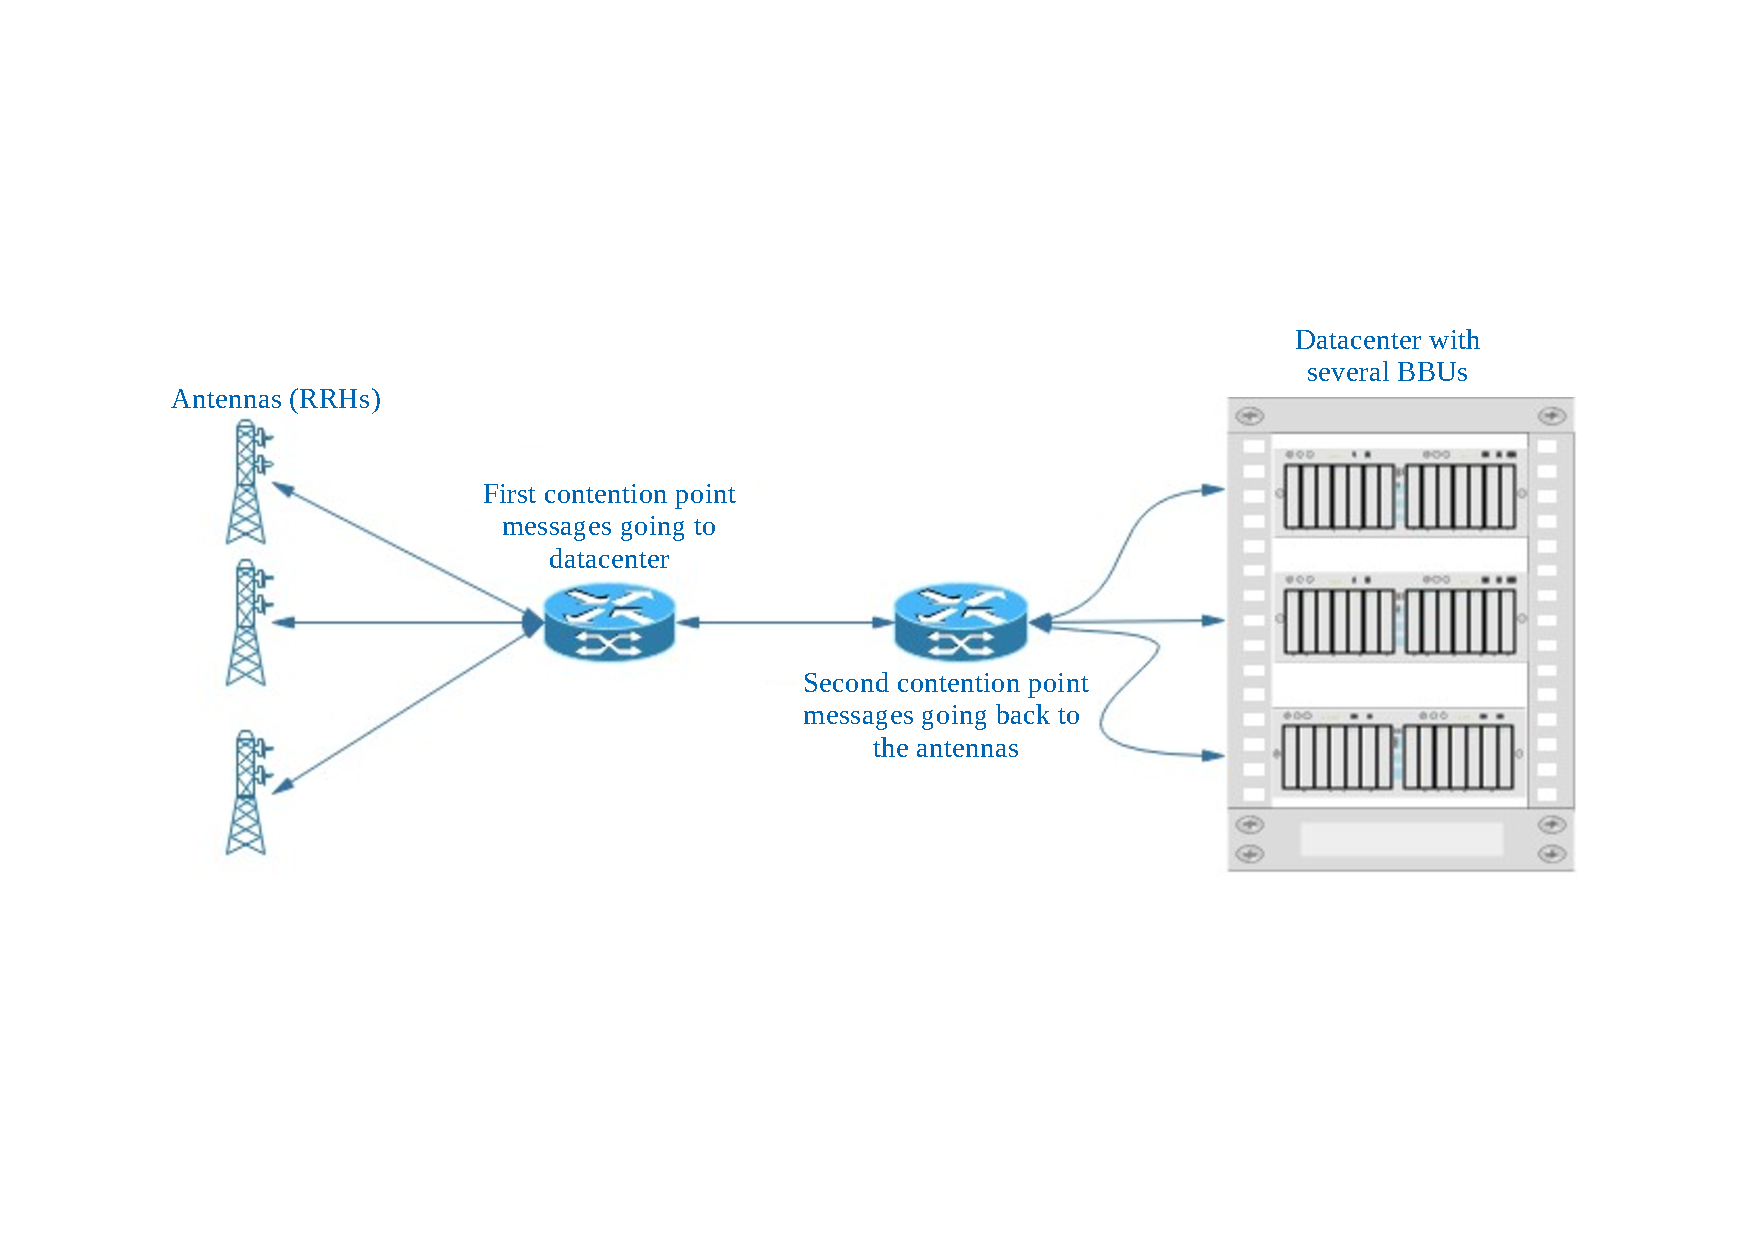
\includegraphics[scale=0.3]{network2.pdf} 
\end{minipage}
\hfill
\begin{minipage}[c]{.45\linewidth}
\centering
\scalebox{0.45}{
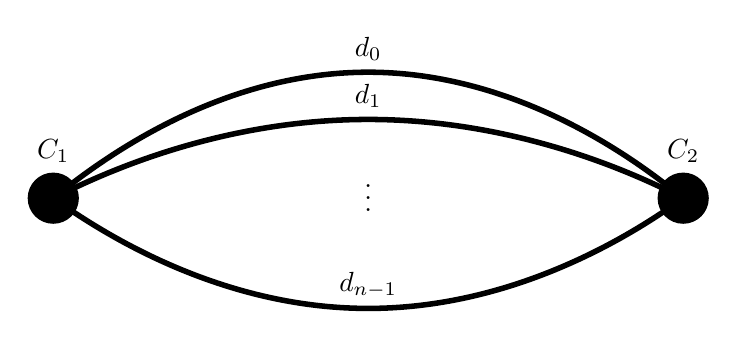
\begin{tikzpicture}
    \SetGraphUnit{5}
      \node[black] at (8,5.9) {$d_0$};
       \node[black] at (4,4.6) {$C_1$};
        \node[black] at (12,4.6) {$C_2$};
         \node[black] at (8,5.3) {$d_1$};
            \node[black] at (8,2.9) {$d_{n-1}$};
            \node[black] at (8,4.15) {.};
            \node[black] at (8,4.0) {.};
            \node[black] at (8,3.85) {.};
  \tikzstyle{VertexStyle}=[shape = circle, draw, minimum size = 10pt]
  \SetUpVertex[FillColor=black]  
  \Vertex[x=4,y=4]{1}
  \Vertex[x=12,y=4]{2}  
 \draw[->,line width=2pt,black] (4,4) parabola bend (8,5.6) (12,4);
  \draw[->,line width=2pt,black] (4,4) parabola bend (8,5) (12,4);
      \draw[->,line width=2pt,black] (4,4) parabola bend (8,2.6) (12,4);
\end{tikzpicture}
}
\end{minipage}
\caption{C-RAN network with a single shared link modeled by two contention points and delays}
\label{fig:model}
\end{figure}
\end{center}
In this article, we model a simple network, as represented in Fig.\ref{fig:model}, in which periodic messages flow through a single bidirectional link. The answer to each message is then sent back through the same link and it does not interact with the messages sent in the other direction, since the link we model is full-duplex. In the C-RAN context we model, all messages are of the same nature, hence they are all the same size denoted by $\tau$. This \textbf{size} represents the time needed to send a message through some contention point of the network, here a link shared by all antennas. We denote by $n$ the number of messages, which are numbered from $0$ to $n-1$. A message $i$ is characterized by its \textbf{delay} $d_i$: when the message number $i$ arrives at the link at time $t$, then it returns to the other end of the link on its way back at time $t + d_i$. 
 The model and problem can easily be generalized to any topology, that is any directed acyclic multigraph with any number of contention points, see \cite{dominique2018deterministic}. We choose here to focus on the simplest, but realistic, non-trivial network, for which we can still obtain some theoretical results. 

The time is discretized and the process we consider is periodic of fixed integer \textbf{period $P$}. We use the notation $[P]$ for the set $\{0,\dots,P-1\}$. Since the process is periodic, we may consider any interval of $P$ units of time and the times at which messages go through the two contention points during this interval to completely represent the state of our system. We call the representation of the interval of time in the first contention point the \textbf{first period} and the \textbf{second period} for the second contention point.

An \textbf{offset} of a message is a choice of time at which it arrives
at the first contention point (i.e. in the first period). Let us consider a message $i$
of offset $o_i$, it uses the interval of time $[i]_1 = \{ (o_i + t) \mod P \mid 0 \leq t < \tau \}$ in the first period and $[i]_2 = \{ (d_i + o_i + t) \mod P \mid 0 \leq t < \tau \}$ in the second period. Two messages $i$ and $j$ \textbf{collide} if either $[i]_1 \cap [j]_1 \neq \emptyset $ or $[i]_2 \cap [j]_2 \neq \emptyset $. If $t \in [i]_1$ (resp. $t \in [i]_2$), we say that message $i$ uses time $t$ in the first period (resp. in the second period).

We want to send all messages, so that there is no collision in the shared link.
In other words, we look for a way to send the messages without using buffering and 
hence limiting the latency of messages to the physical length of the links. An \textbf{assignment} is a
choice of an offset for each message such that \emph{no pair of messages collide}, as shown in Fig.~\ref{fig:assignment}.
Formally, an assignment is a function from the messages in $[n]$ to their offsets in $[P]$.  
Let \textbf{Periodic Message Assignment} or \pma be the following problem: given an instance of $n$ messages, a period $P$ and a size $\tau$, find an assignment or decide there is none. When an assignment is found, we say the problem is solved \textbf{positively}.

\begin{figure}
\begin{center}
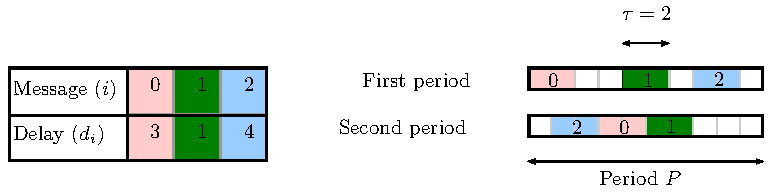
\includegraphics[scale=0.7]{instance}
\end{center}
\caption{An instance of \pma with $3$ messages, $P= 10$, $\tau = 2$, and one assignment}
\label{fig:assignment}
\end{figure}


The complexity of \pma is not yet known. However, we have proven that, when parameterized by
$n$ the number of messages, the problem is \FPT~\cite{barth2018deterministic}.
A slight generalization of \pma, with more contention points but each message only going through two of them, as in \pma, is \NP-hard~\cite{barth2018deterministic}. If the shared link is not full-duplex, that is, there is a single contention point and each message goes through it twice, it is also \NP-hard~\cite{orman1997complexity}. Hence, we conjecture that \pma is \NP-hard.

To overcome the supposed hardness of \pma, we study it when the load of the system is small enough. The \textbf{load} is defined as the number of units of time used in a period by all messages divided by the period that is $n\tau /P$. There cannot be an assignment when the load is larger than one; we prove in this article that, for moderate loads, there is \emph{always} an assignment and that it can be found by a polynomial time algorithm.



\section{Greedy Algorithms for Large Messages} \label{sec:large}

In this section, we study the case of arbitrary values for $\tau$. When modeling real problems,
it is relevant to have $\tau > 1$ when the transmission time of a single message is large with regard to its delay,
which is the case in C-RAN networks.

A \textbf{partial assignment} $A$ is a function defined from a subset $S$ of $[n]$ to $[P]$.
The cardinal of $S$ is the \textbf{size} of partial assignment $A$. A message in $S$ is \textbf{scheduled} (by $A$), and a message not in $S$ is \textbf{unscheduled}. We only consider partial assignments such that no pair of messages of $S$ collide. If $A$ has domain $S$, and $i \notin S$, we define the extension of $A$ to the message $i$ by the offset $o$, denoted by $A[i \rightarrow o]$, as $A$ on $S$ and $A[i \rightarrow o](i) = o$.

All presented algorithms build an assignment incrementally, by growing the size of a partial assignment. Moreover, algorithms of this section are \emph{greedy}: Once an offset is chosen for a message, it is never changed.
In the rest of the paper, we sometimes compare the relative position of messages, but one should remember that the
time is periodic and these are relative positions on a circle. Moreover, when it is unimportant and can hinder comprehension, we may omit to write \emph{mod P} in some definitions and computations.


\subsection{First Fit}


Consider some partial assignment $A$, the message $i$ uses all times from $A(i)$ to $A(i) + \tau -1$ in the first period. If a message $j$ is scheduled by $A$, with $A(j) < A(i)$, then the last time it uses in the first period is $A(j)+\tau-1$ and it should be less than $A(i)$, which implies that $A(j) \leq A(i) - \tau$. Symmetrically, if $A(j) > A(i)$, to avoid collision between messages $j$ and $i$, we have $A(j) \geq A(i) + \tau$. Hence, message $i$ forbids the interval $]A(i) - \tau, A(i) + \tau[$ as offsets for messages still not scheduled, because of its use of time in the first period. The same reasoning shows that $2\tau -1$ offsets are also forbidden because of the times used in the second period. Hence, if $|S|$ messages are already scheduled, then $|S|(4\tau -2)$ offsets are forbidden for any unscheduled message. It is an upper bound on the number of forbidden offsets, since the same offset can be forbidden twice because of a message on the first and on the second period.

Let $Fo(A)$ be the maximum number of forbidden offsets when extending $A$. Formally, assume $A$ is defined over $S$ and $i\notin S$, $Fo(A)$ is the maximum over all possible values of $d_i$ of $|\left\{ o \in [P] \mid A[i \rightarrow o] \text{ has no collision}\right\}|$. The previous paragraph shows that $Fo(A)$ is always bounded by $(4 \tau -2)|S|$. 

Let \firstfit be the following algorithm:  for each unscheduled message (in the order they are given), it tests all offsets from $0$ to $P-1$ until one does not create a collision with the current assignment, and use it to extend the assignment. If $Fo(A) < P$, then whatever the delay of the route we want to extend $A$ with, there is an offset to do so. Since $Fo(A) \leq (4 \tau -2)|S|$ and $|S| < n$, \firstfit (or any greedy algorithm) will always succeed when $(4 \tau -2)n \leq P$, that is when the load $ n\tau /P$ is less than $1/4$.
It turns out that \firstfit always creates compact assignments (as defined in~\cite{dominique2018deterministic}), that is a message is always next to another one in one of the two periods. Hence, we can prove a better bound on $Fo(A)$, when $A$ is built by \firstfit, as stated in the following theorem.

\begin{theorem}
\firstfit solves \pma positively on instances of load less than $1/3$. 
\end{theorem}
\begin{proof}
We show by induction on the size of $S$, that $Fo(A) \leq |S|(3\tau -1) + \tau -1$. For $S = 1$, it is clear since a single message forbid at most $(3\tau -1) + \tau -1 = 4\tau-2$ offsets, as explained before. Now, assume $Fo(A) \leq |S|(3\tau -1) + \tau -1$ and consider a route $i \notin S$ such that \firstfit builds $A[i \rightarrow o]$ from $A$. By definition of \firstfit, choosing $o-1$ as offset creates a collision. W.l.o.g. say it is a collision in the first period. It means that there is a scheduled message between $o - \tau $ and $o-1$, hence all these offsets are forbidden by $A$. The same offsets are also forbidden by the choice of $o$ as offset for $i$, then only $3\tau -1$ new offsets are forbidden, that is $Fo(A[i \rightarrow o]) \leq Fo(A) + (3\tau -1)$, which proves the induction and the theorem.
\end{proof}

\subsection{Meta-Offset}

The method of this section is described in~\cite{dominique2018deterministic} and it achieves the same bound on the load using a different method. It is recalled here to help understand several algorithms in the article.
The idea is to restrict the possible offsets at which messages can be scheduled. It seems counter-intuitive, since it decreases artificially the number of available offsets to schedule new messages. However, it allows reducing the number of forbidden offsets for unscheduled messages. A \textbf{meta-offset} is an offset of value $i\tau$,
with $i$ an integer from $0$ to $P / \tau$. We call \metaoffset the greedy algorithm which works as \firstfit, but consider only meta-offsets when scheduling messages. 

Let $Fmo(A)$ be the maximal number of meta-offsets forbidden by $A$. 
 By definition, two messages with a different meta-offset cannot collide in the first period.
Hence, $Fmo(A)$ can be bounded by $3|S|$ and we obtain the following theorem.


\begin{theorem}[Proposition 3 of~\cite{dominique2018deterministic}]
\metaoffset solves \pma positively on instances of load less than $1/3$.
\end{theorem}

The complexity of a naive implementation of \metaoffset is in $O(n P/\tau)$, while \firstfit is in $O(nP)$. However, it is not useful to consider every possible (meta-)offset at each step. By maintaining a list of increasing position of scheduled messages in first and second period, both algorithms can be implemented in time $O(n^2)$.

\subsection{Compact Tuples}

We present in this section a family of greedy algorithms which solve \pma positively for larger loads. We try to combine the good properties of the two previous algorithms: the compactness of the assignments produced by \firstfit and the absence collision in the first period of \metaoffset. The idea is to schedule several messages at once, using meta-offsets, to maximize the compactness of the obtained solution. We first describe the algorithm which schedules pairs of routes and then explain quickly how to extend it to any tuples of messages.


From now on, we use Lemma~\ref{lemma:multiple} to assume $P = m\tau$. This hypothesis makes the analysis of algorithms based on meta-offsets simpler and tighter. The load increases from $\lambda = n \tau / P$ to at most $\lambda (1 + 1/m)$: the difference is less than $1/m < 1/n$, thus very small for most instances. The transformation of Lemma~\ref{lemma:multiple} does not give a bijection between assignments of both instances but only an injection, which is enough for our purpose. 

\begin{lemma}\label{lemma:multiple}
Let $I$ be an instance of \pma with $n$ messages of size $\tau$, period $P$ and $m = \lfloor P / \tau \rfloor$. There is an instance $J$ with $n$ messages of size $\tau'$ and period $P'= m\tau'$ such that any assignment of $J$ can be transformed into an assignment of $I$ in polynomial time.
\end{lemma}
\begin{proof}
%Fig.~\ref{fig:multipleperiod} illustrates the reductions we define in this proof on a small instance.
Let $P = m \tau + r$ with $r \leq \tau$. We define the instance $I'$ as follows: $P' = mP$, $d_{i}' = m d_i$ and $\tau' = m \tau + r$. With this choice, we have $P' = m(m \tau + r) = m \tau'$.
Consider an assignment $A'$ of the instance $I'$.
If we let $\tau'' = m\tau$, then $A'$ is also an assignment for $I'' = (P',\tau'',(d_{0}',\dots,d_{n-1}'))$. Indeed, the size of each message, thus the intervals of time used in the first and second period begin at the same position but are shorter, which cannot create collisions. We then use a compactification procedure on $A'$ seen as an assignment of $I''$,
with size of messages multiple of $m$ (see Th.4 of~\cite{dominique2018deterministic} for a similar compactification). W.l.o.g., the first message is positioned at offset zero. The first time it uses in the second period is a multiple of $m$ since its delay is by construction a multiple of $m$. Then, all other messages are translated to the left by removing increasing values to their offsets, until there is a collision. It guarantees that some message $j$ is in contact with the first one on the first or second period. It implies that either $A'(j)$ or $A'(j)+d_j \mod P'$ is a multiple of $m$ and since $d_j$ is a multiple of $m$, then both $A'(j)$ and $A'(j)+d_j \mod P'$ are multiples of $m$. This procedure can be repeated until we get an assignment $A''$ to $I''$, such that all positions of messages in the first and second period are multiples of $m$. Finally, we define $A$ as $A(i) = A''(i)/m$ and we obtain an assignment of $I$. 
\end{proof}

%\begin{figure}
% \begin{center}
%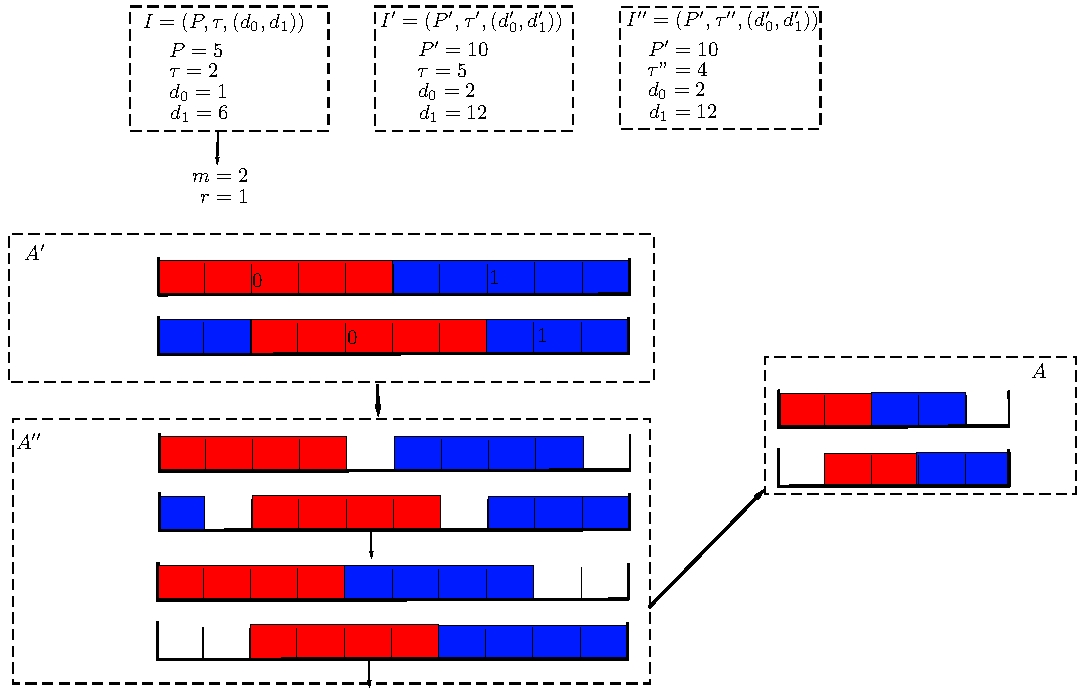
\includegraphics[scale=0.75]{multipleperiod}
%\end{center}
%\caption{Transformation from $A''$ to $A$}
%\label{fig:multipleperiod}
%\end{figure}


We are interested in the remainder modulo $\tau$ of the delays, let $d_i = d_{i}'\tau + r_i$ be the Euclidean division of $d_i$ by $\tau$. We assume, from now on, that \emph{messages are sorted by increasing $r_i$}.
A \textbf{Compact pair}, as shown in Fig.~\ref{fig:compactpair} is a pair of messages $(i,j)$ with $i < j$ that can be scheduled using meta-offsets such that $A(i) + (d'_i+1)\tau = A(j) + d'_j\tau$, i.e. $j$ is positioned less than $\tau$ unit of times after $i$ in the second period.
The \textbf{gap} between $i$ and $j$ is defined as  $g = d_{i}' + 1 - d'_{j} \mod m$, it is the distance in meta offsets between $i$ and $j$ in the first period. By definition, we can make a compact pair out of $i$ and $j$, if and only if their gap is not zero.

\begin{figure}[h]
\begin{center}

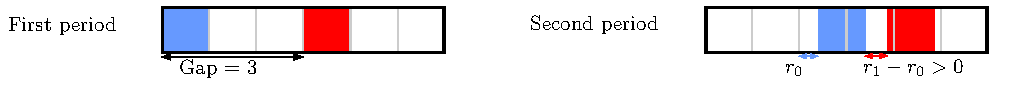
\includegraphics[scale=0.7]{compact_pair}
\end{center}
\caption{A compact pair scheduled using meta-offsets, with $d'_0 = 2$ and $d'_0 = 0$}
\label{fig:compactpair}
\end{figure}

\begin{lemma}\label{lemma:pair_find}
Given three messages, two of them form a compact pair. 
\end{lemma}
\begin{proof}
If the first two messages or the first and the third message form a compact pair,
then we are done. If not, then by definition $d_{1}' = 1 + d_{2}' = 1 + d_{3}'$. Hence, messages $2$ and $3$ have the same delay and form a compact pair of gap $1$.
\end{proof}

Let \compactpair be the following greedy algorithm: From the messages in order
of increasing $r_i$, a sequence of at least $n/3$ compact pairs is built using Lemma~\ref{lemma:pair_find}. Pairs are scheduled in the order they have been built using meta-offsets. If at some point all compact pairs are scheduled or the current one cannot be scheduled, the remaining messages are scheduled as in \metaoffset. The analysis of \compactpair relies on the evaluation of the number of forbidden meta-offsets. In the first phase of \compactpair, one should evaluate the number of forbidden offsets when scheduling a compact pair, that we denote by $Fmo_2(A)$. In the second phase, we need to evaluate $Fmo(A)$. When scheduling a message in the second phase, a scheduled compact pair only forbids \emph{three} meta-offsets in the second period. If messages in a pair are scheduled independently, they forbid \emph{four} meta-offsets, which explains the improvement from \compactpair. We first state a simple lemma, whose proof can be read from Fig.~\ref{fig:forbidenmeta}, which allows bounding $Fmo_2(A)$.

\begin{lemma}\label{lemma:pair_forbid}
A compact pair already scheduled by \compactpair forbids at most four meta-offsets in the second period to another compact pair when scheduled by \compactpair.
\end{lemma}

\begin{figure}
\begin{center}
\includegraphics[scale=0.7]{pairforbiden}
\end{center}

\caption{Meta offsets forbidden by a scheduled compact pair (in blue) when scheduling another compact pair (in red)} 
\label{fig:forbidenmeta}
\end{figure}
\begin{theorem}
\compactpair solves \pma positively on instances of load less than
$3/8$.
\end{theorem}
\begin{proof}
Let $n_2$ be the number of compact pairs scheduled in the first phase. When scheduling a new pair, the position of the $2n_2$ messages on the first period forbid $4n_2$ offsets for a compact pair. Indeed, each scheduled message can collide
with each of the two messages which form a compact pair. On the second period, we can use Lemma~\ref{lemma:pair_forbid} to bound the number of forbidden offsets by $4n_2$. 
Hence, we have established that during the first phase, the partial solution $A$
satisfies $Fmo_2(A) \leq 8n_2$. This first phase continues while there are available offsets for compact pairs, which is guaranteed when $Fmo_2(A) \leq m$, that is while $n_2 \leq m/8$. Hence, we assume that $n_2 = m/8$.

In the second phase, a compact pair forbids $3$ meta offsets in the 
second period and $2$ in the first. Hence, if we let $n_1$ be the number of messages scheduled in the second phase to build partial assignment $A$, we have $Fmo(A) \leq n_2*5 + n_1*3$. 
\compactpair can always schedule messages when $Fmo(A)$ is less than $m$, which is implied by $n_2*5 + n_1*3 \leq m$.
Solving this equation, we obtain that $n_1 \geq \frac{m}{8}$ thus the number of routes scheduled is at least $2n_2 + n_1 \geq \frac{3}{8}m$. Assuming there are exactly $\frac{3}{8}m$ messages to schedule, then $\frac{2m}{8}$ messages are scheduled as compact pairs. It is two third of the $\frac{3}{8}m$ messages, hence Lemma~\ref{lemma:pair_find} guarantees the existence of enough compact pairs. Therefore, an assignment is always produced when the load is less or equal to $\frac{3}{8}$.
\end{proof}

\compactpair can be improved by forming compact tuples instead of compact pairs.
A compact $k$-tuple is a sequence of messages $i_1 < \dots < i_k$ (with $r_{i_1},\dots,r_{i_k}$ increasing), for which meta-offsets can be chosen so that, there is no collision, the messages in the second period are in order $i_1,\dots,i_k$ and for all $l$, $A(i_l) + (d'_{i_l} + 1)\tau = A(i_{l+1}) + d'_{i_{l+1}}\tau$.
The algorithm \texttt{Compact k-tuples} works by scheduling compact $k$-tuples
using meta offsets while possible, then scheduling compact $k-1$-tuples and so on until $k=1$.


\begin{lemma}\label{lemma:uple_find}
Given $k + k(k-1)(2k-1)/6$ messages, $k$ of them always form a compact $k$-tuple and we can find them in polynomial time. 
\end{lemma}
\begin{proof}
We prove the property by induction on $k$. We have already proved it for $k=2$ in Lemma~\ref{lemma:pair_find}.
Now assume that we have found $C$ a compact $(k-1)$-tuple in the first $(k-1)^3/3$
messages. Consider the next $(k-1)^2 + 1$ messages. If $k$ of them have the same delay modulo $\tau$,
then they form a compact $k$-tuple and we are done. Otherwise, there are at least $k$ different values modulo $\tau$
in those $(k-1)^2 + 1$ messages. Each element of the compact $(k-1)$-tuple forbids one value for the delay modulo $\tau$ of a new $k$th element in the tuple. By pigeonhole principle, one of the $k$ messages with distinct delays modulo $\tau$ can be used to extend $C$. We have built a compact $k$-tuple from at most $(k-1) + (k-1)(k-2)(2k-3)/6 + (k-1)^2 + 1$ messages.
It is equal to $k + k(k-1)(2k-1)/6$ which proves the induction.
\end{proof}


\begin{theorem}\label{th:k-tuples}
\texttt{Compact 8-tuples} always solves \pma positively on instances of load less than $4/10$, for instances with $n \geq 220$.
\end{theorem}
\begin{proof}
We need the following fact, which generalizes Lemma~\ref{lemma:pair_forbid}: A $k$-tuples forbids $k+j+1$ offsets in the second period when scheduling a $j$-tuple. %If the remainder of the messages in the $j$-tuples are larger than the remainder in the $k$-tuples, it forbids $k+j$ messages only.
It enables us to compute a lower bound on the number of scheduled $i$-tuples for $i$ equal $k$ down to $1$ by bounding $Fmo_i(A)$, the number of forbidden meta-offsets when placing $i$-tuple in the algorithm.
If we denote by $n_i$ the number of compact $i$-tuples scheduled by the algorithm,
we have the following equation:  $$ Fmo_i(A) \leq \displaystyle{\sum_{j=i}^k n_j(j*i + j + i+ 1)}.$$
The equation for $n_1$ is slightly better: 
$$ Fmo(A) \leq \displaystyle{\sum_{j=1}^k n_j(2j + 1)}.$$
A bound on $n_i$ can be computed, using the fact that $A$ can be extended while $Fmo_i(A) < m$. 
Lemma~\ref{lemma:uple_find} ensures there are enough compact $k$-tuples, when $n - \sum_{j \leq i \leq 8} n_j$ is larger than $i + i(i-1)(2i-1)/6$. 
A numerical computation of the $n_i$'s shows that \texttt{Compact 8-tuples} always finds an assignment when the load is less than $4/10$ and for $n \geq 220$.
\end{proof}

Th.~\ref{th:k-tuples} is obtained for $k=8$. Taking arbitrary large $k$ and using refined bounds on $Fmo_i(A)$ is not enough to get an algorithm working for a load of $41/100$ (and it only works from larger $n$).

The code computing the $n_i$ can be found on one author's website\footnote{\url{https://yann-strozecki.github.io/}}.
To make \texttt{Compact 8-tuples} work, there must be at least $220$ messages to
produce enough compact $8$-tuples in the first phase. It is not a strong restriction for two reasons. First, the bound of Lemma~\ref{lemma:uple_find} can be improved, using a smarter polynomial time algorithm to find compact tuples, which better takes into account repetitions of values and compute the compact tuples in both directions. Second, on random instances, the probability that $k$ messages do not form a compact $k$-tuples is low, and we can just build the tuples greedily. Therefore, for most instances, forming compact $k$-uples is not a problem and in practice \texttt{Compact 8-tuples} works even for small $n$.

\section{Messages of Size One} \label{sec:small}

When $\tau = 1$ and the load is less than $1/2$, \emph{any greedy algorithm} solves \pma positively since $Fo(A) \leq (4\tau -2)|S| = 2|S|$ where $S$ is the number of scheduled messages. We give, in this section, a method which always finds an assignment for sometimes load larger than $1/2$.

\subsection{Deterministic Algorithm}

To go above $1/2$ of load, we optimize a potential measuring how many offsets are available for all messages, scheduled or not. Messages are scheduled while possible using any greedy algorithm. Then, when all unscheduled messages have no available offset, we use a Swap operation defined later, which improves the potential. When the potential is high enough, it ensures that there are two messages whose offset can be changed so that a new message can be scheduled. 

The algorithm is not greedy, since we allow to exchanging a scheduled message with an unscheduled one. It cannot work online, since it requires to know all delays of the messages in advance. 

\begin{definition}
The potential of a message of delay $d$, for a partial assignment $A$
is the number of integers $i \in [P]$ such that $i$ is used in the first period and $i+d \mod P$ is used in the second period.
\end{definition}

%The computation of the potential of a message of delay $3$, is illustrated in Fig.~\ref{fig:messagepotential}.
The potential of a message counts the configurations which reduce the number of forbidden offsets.
Indeed, when $i$ is used in the first period and $i+d \mod P$ is used in the second period,
then the same offset is forbidden \emph{twice} for a message of delay $d$. Hence, the potential of a message is related to the number of possible offsets as stated in the following lemma. 
%\begin{figure}
% \begin{center}
%\includegraphics[scale=1]{messagepotential}
%\end{center}
%\caption{A message with a potential $2$}
%\label{fig:messagepotential}
%\end{figure}

\begin{lemma}
Given a partial assignment $A$ of size $s$, and $i$ an unscheduled message of potential 
$v$, then the set $\{o \mid A(i \rightarrow o) \text{ has no collision}\}$ is of size $P - 2s + v$.
\end{lemma}

For our algorithm, we need a global measure of quality of a partial assignment, 
that we try to increase when the algorithm fail to schedule new messages. 
We call our measure \textbf{the potential of an assignment} and we denote it by $Pot(A)$, it is the sum of potentials of all messages in the instance.


\begin{definition}
The potential of a position $i$, for a partial assignment $A$, is the number of messages of delay $d$ such that $i+d \mod P$ is used by a route scheduled by $A$. 
\end{definition}

%\begin{figure}
% \begin{center}
%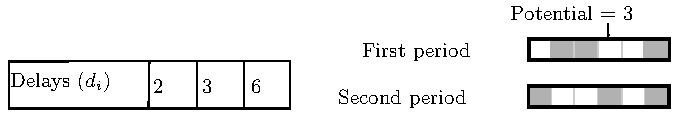
\includegraphics[scale=1]{positionspotential}
%\end{center}
%\caption{A position of potential $3$}
%\label{fig:positionpotential}
%\end{figure}

%The potential of a position is illustrated in Fig.~\ref{fig:positionpotential}.
Instead of decomposing the global potential as a sum over messages, it can be understood
as a sum over positions, as stated in the next lemma.

\begin{lemma}\label{lemma:pot_pos}
The sum of potentials of all positions used in the first period by messages scheduled by $A$ is equal to $Pot(A)$.  
\end{lemma}

By definition of the potential of a position, we obtain the following simple invariant.

\begin{lemma}\label{lemma:inv}
The sum of potentials of all positions for a partial assignment with $k$ scheduled messages is $nk$.  
\end{lemma}

 As a consequence of this lemma, $Pot(A) \leq nk$. Let us define a \textbf{Swap operation},
 which guarantees to obtain at last half the maximal value of the potential.
Let $A$ be some partial assignment of size $s$ and let $i$ be an unscheduled message of delay $d$. 
Assume that $i$ cannot be used to extend $A$. The Swap operation is the following: 
select a free position $o$ in the first period, remove the message which uses the position $o+d$ in the second period from $A$ and extend $A$ by $i$ with offset $o$. We denote this operation by $Swap(i,o,A)$.

\begin{lemma}\label{lemma:swap}
Let $A$ be some partial assignment of size $k$ and let $i$ be an unscheduled message. If $i$ cannot be used to extend $A$, then either $Pot(A) \geq kn/2$ or there is an $o$ such that $Pot(Swap(i,o,A)) > Pot(A)$.
\end{lemma}

\begin{proof}
The positions in the first period can be partitioned into $P_{u}$ the positions used by some scheduled message and $P_{f}$ the positions unused.
Let $V_f$ be the sum of the potentials of the positions in $P_f$ and let $V_u$ be the sum of the potentials of the positions in $P_u$. By Lemma~\ref{lemma:inv}, since $P_f$ and $P_u$ partition the positions, we have $V_f + V_u = kn$. Moreover, by Lemma~\ref{lemma:pot_pos}, $Pot(A) = V_u$, then $V_f + Pot(A) = kn$.

By hypothesis, $i$ cannot be scheduled, then, for all $p \in P_{f}$, $p+d_i$ is used in the second period. Let $F$ be the function which associates to $p \in P_{f}$ the position $A(j)$ such that there is a scheduled route $j$ which uses $p+d_i$ in the second period, that is $A(j) + d_j = p + d_i \mod P$. The function $F$ is an injection from $P_{f}$ to $P_u$. Remark that, in both $Swap(i,p,A)$ and $A$, exactly the same positions are used in the second period. Hence, the potential of each position stay the same after the swap. As a consequence, doing the operation $Swap(i,p,A)$ adds to $Pot(A)$ the potential of the position $p$ and removes the potential of the position $F(p)$. 

Assume now, to prove our lemma, that for all $p$, $Pot(Swap(i,p,A)) \leq Pot(A)$. It implies that for all $p$, the potential of $p$ is smaller than the potential of $F(p)$. Since $F$ is an injection from $P_f$ to $P_u$, we have that $V_f \leq V_u = Pot(A)$. Since $V_f + Pot(A) = kn$, we have that $Pot(A) \geq kn/2$.
\end{proof}

%\subsubsection*{The Swap Algorithm}


Let us precisely describe the algorithm \swapandmove:  messages are scheduled while possible by \firstfit and then the Swap operation is applied while it increases the potential. When the potential is maximal, \swapandmove schedule a new message by moving at most two scheduled messages to other available offsets. If it fails to do so, \swapandmove stops, otherwise the whole procedure is repeated. We analyze \swapandmove in the following theorem.

\begin{theorem}
\swapandmove solves positively \pma, in polynomial time, for instances with $\tau =1$ and load less than $1/2 + (\sqrt{5}/2 -1) \approx 0,618$.
\end{theorem}

\begin{proof}
We determine for which value of the load \swapandmove always works. We let $n = (1/2 + \epsilon)P$ be the number of messages, the load is $1/2 + \epsilon$. We need only to study the case when $n-1$ messages are scheduled by $A$ and \swapandmove tries to schedule the last one, since the previous steps are similar but easier. 

Let $d$ be the delay of the unscheduled message. We consider the pairs 
of times $(o,o+d)$ for $o \in [P]$. Since the message
cannot be scheduled, there are three cases. First, $o$ is unused in the first period but $o+d$ is used in the second period. Since there are $n-1$ scheduled messages, there are $P-n+1$ such value of $o$. If a message using the time $o+d$ in the second period can be scheduled elsewhere, so that the unscheduled message can use offset $o$, then \swapandmove succeeds.
Otherwise, the message has no possible offsets, which means its potential is equal to $2(\epsilon P -1)$.
The second case is symmetric: $o$ is used in the first period but $o+d$ is unused in the second period. 
Finally, we have the case $o$ is used in the first period and $o+d$ is used in the second period.  There are $2(\epsilon P -1)$ such values of $o$. If the two messages using times 
$o$ and $o+d$ can be rescheduled so that offset $o$ can be used for the unscheduled message,
then \swapandmove succeeds. This is always possible when one message is of potential at least $2\epsilon P -1$ and the other of potential at least $2\epsilon P + 1$. Since the messages must be of potential more than $2(\epsilon P -1)$ and at most $n-1$, it is satisfied when the sum of the two potentials is at least $2(\epsilon P -1) + n$.

If we assume that \swapandmove was unable to schedule the last message by moving two scheduled messages, the previous analysis gives us a bound on twice $Pot(A)$: 
$$ 2Pot(A) \leq 2(P-n+1) 2(\epsilon P -1) + 2(\epsilon P -1)(2(\epsilon P -1) + n) $$
$$ Pot(A) \leq (\epsilon P -1) (P + n)$$
By Lemma~\ref{lemma:swap}, we know that $Pot(A) \geq n(n-1)/2$, hence 
\swapandmove must succeed when
$$n(n-1)/2 \geq  (\epsilon P -1) (P + n).$$
By expanding and simplifying, we obtain a second degree inequation in $\epsilon$, $1/4 - 2\epsilon - \epsilon ^2 \geq  0$.
Solving this inequation yields $\epsilon \leq \sqrt{5}/2 -1$.


Let us prove that \swapandmove is in polynomial time. All Swap operations 
strictly increase the potential. Moreover, when one or two messages are moved, the potential may decrease but
a message is added to the partial assignment. The potential is bounded by $O(n^2)$ and the move operations all together can only remove $O(n^2)$ to the potential, hence there are at most $O(n^2)$ Swap operations during \swapandmove. A Swap operation can be performed in time $O(n)$, since for a given message, all free offsets must be tested and the potential is evaluated in time $O(1)$ (by maintaining the potential of each position). This proves that Swap and Move is in $O(n^3)$.  
\end{proof}

Consider a partial assignment of size $n' = (1/2 + \epsilon)P$, and a message of delay $d$.
If we consider all $n'$ used offsets $o$ and all times time $o+d$ in the second period, 
then $o$ and $o+d$ are both used for at least $n' - (P -n') = 2\epsilon P$ values of $o$.
The potential of any message is thus larger or equal to $2\epsilon P$. When a message cannot be scheduled, its potential is less or equal to $2\epsilon P$, hence it is equal to $2\epsilon P$.

Hence, the potential of any assignment of size $n'$ is at least $2\epsilon P n $. As a consequence, the method of Lemma~\ref{lemma:swap} will guarantee a non-trivial potential for $2\epsilon P n <  nn'/2$, that is $\epsilon < 1/6$. Any algorithm relying on the potential and the Swap operation cannot be guaranteed to work for load larger than $2/3 = 1/2 + 1/6$. However, we may hope to improve on the analysis of Lemma~\ref{lemma:swap}, since it is not optimal: $2\epsilon P$ positions in $P_{u}$ are not taken into account in the proof. 

We conjecture that \swapandmove works for load up to $2/3$. 
On random instances, we expect the potential to be higher than the stated bound and to be better spread on the messages, which would make \swapandmove works for larger loads, as it is indeed observed in experiments (see Appendix~\ref{sec:perf_small}).

\subsection{Randomized Algorithm for Random Instances}

We would like to understand better the behavior of our algorithms
on instances drawn uniformly at random. To this aim, we analyze the algorithm \greedyuniform, defined as follows: for each message in the order of the input, choose one of the offsets, which does not create a collision with the current partial assignment, uniformly at random. 

We analyze \greedyuniform over random instances:  all messages have 
their delays drawn independently and uniformly in $[m]$. We compute the probability of success of \greedyuniform over all random choices by the algorithm \emph{and all possible instances}. 
It turns out that this probability, for a fixed load strictly less than one, goes to one when $m$ grows. 
For a given partial assignment, we are only interested in its trace: the set of times which are used in the first and second period. Hence, if $n$ messages are scheduled in a period of size $m$, the trace of an assignment is a pair of subsets of $[m]$ of size $n$. We now show that these traces are produced uniformly by \greedyuniform.

\begin{theorem}
The distribution of traces of assignments produced by \greedyuniform when it succeeds, from instances drawn uniformly at random, is also uniform.
\end{theorem}
\begin{proof}
The proof is by induction on $n$, the number of messages. It is clear for $n=1$,
since the delay of the first message is uniformly drawn and all offsets can be used.
Assume now the theorem true for some $n>1$. \greedyuniform, by induction hypothesis has produced
uniform traces from the first $n$ messages.  Hence, we should prove that, if we draw the delay
of the $n+1^{th}$ message randomly, extending the trace by a random possible offset produces a random distribution on the traces of size $n+1$. 

 If we draw an offset uniformly at random (among all $m$ offsets) and then extend the trace by scheduling the last message at this offset or fail, the distribution over the traces of size $n+1$ is the same as what produces \greedyuniform. Indeed, all offsets which can be used to extend the trace have the same probability to be drawn. Since all delays are drawn independently, we can assume that, given a trace, we first draw an offset uniformly, then draw uniformly the delay of the added message and add it to the trace if it is possible. This proves that all extensions of a given trace are equiprobable. Thus, all traces of size $n+1$ are equiprobable, since they each can be formed from $(n+1)^2$ traces of size $n$ by removing one used time from the first and second period. This proves the induction and the theorem.
\end{proof}

Since \greedyuniform can be seen as a simple random process on traces by Th.~\ref{theorem:uniform}, it is easy to analyze its probability of success.

\begin{theorem}\label{theorem:uniform}
The probability over all instances with $n$ messages and period $m$ that \greedyuniform solves $\pma$ positively is $$\displaystyle{\prod_{i=m/2}^{n-1}(1 - \frac{\binom{n}{2i-m}}{\binom{m}{i}})}.$$
\end{theorem}
\begin{proof}
We evaluate $\Pr(m,n)$ the probability that \greedyuniform fails at the $n^{th}$ step assuming it has not failed before. It is independent of the delay of the $n^{th}$ message. Indeed, the operation which adds one to all times used 
in the second period is a bijection on the set of traces of size $n-1$. It is equivalent to remove one to the delay of the $n^{th}$ message. We can thus assume that the delay is zero.

Let $S_1$ be the set of times used in the first period by the $n-1$ first messages
and $S_2$ the set of times used in the second period. We can assume that $S_1$ is fixed, since all subsets of the first period are equiprobable and because $S_2$ is independent of $S_1$ (Th.~\ref{theorem:uniform}). There is no possible offset for the $n^{th}$ message, if and only if $S_1 \cup S_2 = [m]$. It means that $S_2$ has been drawn such that it contains $[m] \setminus S_1$. By Th.\ref{theorem:uniform}, $S_2$ is uniformly distributed over all sets of size $n-1$. Hence, the probability that  $[m]  \setminus S_1 \subseteq S_2$  is the probability to draw a set of size $n-1$ which contains $m-n + 1$ fixed elements. This proves $\Pr(m,n) = \frac{\binom{n}{2(n-1)-m}}{\binom{m}{n-1}}$.

From the previous expression, we can derive the probability of success of \greedyuniform by a simple product of 
the probabilities of success $(1 - \Pr(m,i))$ at step $i$, for all $i \leq n$, which proves the theorem. 
\end{proof}


If we fix the load $\lambda = n/m$, we can bound $P(m,n)$ using Stirling formula. We obtain for some constant $C$, 
that $P(m,n) \leq C \left(\frac{\lambda^{2\lambda}}{(2\lambda -1)^{2\lambda -1}}\right)^m$.
We let $f(\lambda) = \frac{\lambda^{2\lambda}}{(2\lambda -1)^{2\lambda -1}}$.
The derivative of $f$ is strictly positive for $1/2 < \lambda < 1$ and $f(1) = 1$, hence 
$f(\lambda) < 1$ when $\lambda < 1$. By a simple union bound, the probability that \greedyuniform fails is bounded 
by $C \lambda m f(\lambda)^m$, whose limit is zero when $m$ goes to infinity. 
It explains why \greedyuniform is good in practice for large $m$. 


%\section{Conclusion}

%In this article, we have proved that there is always a solution to \pma and that it can be found in polynomial time 
%for large $\tau$ and load  $0.4$ or for $\tau = 1$ and load $0.61$. Moreover, the performance of the presented algorithms over average instances are shown to be excellent empirically but also theoretically for \compactpair.
%Hence, we can use the simple algorithms presented here to schedule C-RAN messages \emph{without buffer nor additional latency}, if we are willing to use only half the bandwidth of the shared link. 

%Many questions on \pma are still unresolved, the first one being its complexity.
%Moreover, we plan to adapt the Swap algorithm to the case $\tau > 1$. While the potential
%can be defined in the same way, it is not yet clear that it would help as much in this setting.
%We could also analyze the behavior of the presented algorithms over random instances in the case $\tau > 1$.
%For instance, it is possible to form very long compact tuples over random instances and we could
%use that to obtain an algorithm which works with high probability for load less than $0.5$. 
%First Fit or Meta Offset can easily be adapted to network topologies with more than a single link, but we could also try to adapt Compact Tuples and Swap. Finally, to capture networks carrying several types of messages, it would be interesting to allow for different message sizes, which makes methods using meta-offsets seemingly useless.



%\section{Lower bounds} 

%Pour m=6, on peut toujours placer 5 éléments, que dire pour plus grand ?
%Remarque si tous les delais sont différents, on peut les placer, expliquer ça. 
%Example/family of examples for which some greedy alg fail -> facile pour le first fit
%Example/family of examples with a given load such that there are no feasible solution.

\newpage
\appendix

\label{sec:appendix}


In this appendix, we provide a justification of our interest for the case $\tau = 1$
and experiments on all algorithms presented in the paper over synthetic data.


\section{From Large to Small Messages}\label{sec:reduction}



In this section, we explain how we can trade load or buffering in the network to reduce the size of messages up to $\tau = 1$. This further justifies the interest of Sec.~\ref{sec:small}, where specific algorithms for $\tau = 1$ are given.

\subsection{Message of Size One by Increasing the Load}

We describe here a reduction from an instance of \pma to another one with the same period and number of messages but 
the size of the messages is doubled. This instance is equivalent to an instance with $\tau = 1$, by dividing everything by the message size. Thus we can always assume that $\tau = 1$, if we are willing to double the load.


\begin{theorem}\label{th:double_load}
Let $I$ be an instance of \pma with $n$ messages and load $\lambda$. There is an instance $J$ with $n$ messages of size $1$
and load $2\lambda$ such that an assignment of $J$ can be transformed into an assignment of $I$ in polynomial time.
\end{theorem}
\begin{proof}
From $I = (P,\tau,(d_{0},\dots,d_{n-1}))$, we build $I' = (P, 2\tau, (d_{0}',\dots,d_{n-1}'))$, where $d_i' = d_{i} - (d_{i} \mod 2\tau)$. The instance $I'$ has a load twice as large as $I$.
On the other hand, all its delays are multiples of $2\tau$ hence solving \pma on $I'$ is equivalent to solving it on $I'' = (P/2\tau, 1,(d_{0}/ 2\tau,\dots,d_{n-1} /2\tau))$, as already explained in the proof of Lemma~\ref{lemma:multiple}. 

Let us prove that an assignment $A'$ of $I'$ can be transformed into an assignment $A$ of $I$. 
Consider the message $i$ with offset $A'(i)$, it uses all times between $A'(i)$ and $A'(i) + 2\tau -1$ in the first period and all times between $A'(i) + d_{i} - (d_{i} \mod 2\tau)$ to $A'(i) + 2\tau -1+ d_{i} - (d_{i} \mod 2\tau)$ in the second period. 
If $d_{i} \mod 2\tau < \tau $, we set $A(i) = A'(i)$, and the message $i$ of $I$ is scheduled ``inside'' the 
message $i$ of $I'$, see Fig.~\ref{fig:transf_2tau}. If $\tau \leq d_{i} \mod 2\tau < 2\tau$, then we set 
$A(i) = A'(i) - \tau$. There is no collision in the assignment $A$, since all messages in the second period use
times which are used by the same message in $A'$. In the first period, the messages scheduled by $A$ use either the first
half of the same message in $A'$ or the position $\tau$ before, which is either free in $A'$ or the second half of the times used by another message in $A'$ and thus not used in $A$. 
\end{proof}
\begin{figure}[h]
\begin{center}

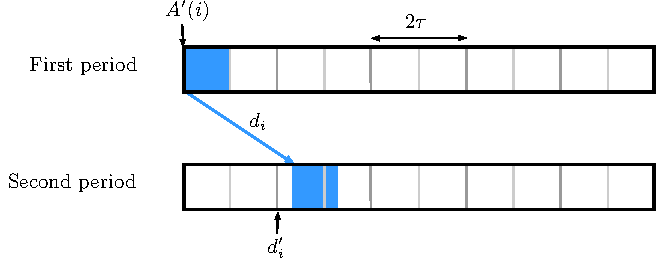
\includegraphics[scale=0.7]{transfo2tau}
\end{center}
\caption{Building $I$ from $I'$}
\label{fig:transf_2tau}
\end{figure}

Remark that combining Greedy Random and Th.~\ref{th:double_load} allows to solve $\pma$ on random instances,
with probability one when the number of routes goes to infinity and the load is strictly less than $1/2$. 
This explains why we have not presented nor analyzed in details an algorithm designed for arbitrary $\tau$ on random instances, since any greedy algorithm, relying on optimizing $Fo(A)$, cannot guarantee anything for load larger than $1/2$.
However, in Sec.~\ref{sec:perf_large}, we present Compact Fit, a simple greedy algorithm which exhibits good performance on random instances.

\subsection{Trade-off between Latency and Message Size}

The problem \pma is simplified version of the practical problem we adress, allowing a single degree of freedom for each message: its offset. If we relax it slightly to be more similar to what is studied in~\cite{barth2018deterministic}, we allow buffering a message $i$ during a time $b$ between the two contention points, which translates here into changing $d_i$ to $d_i + b$. The quality of the solutions obtained for such a modified instance of \pma are worst since the buffering adds latency to the messages. We now describe how we can make a trade-off between the added latency and the size of the messages, knowing that having smaller messages helps to schedule instances with higher load.


The idea is to buffer all messages so that their $d_i$ have the same
remainder modulo $\tau$. It costs at most $\tau - 1$ of buffering, which is not
so good, since algorithms optimizing the latency do better on random instances, see~\cite{barth2018deterministic}. However, it is much better than buffering for a time $P$, the only value for which we are guaranted to find an assignment, whatever the instance. When all delays are changed so that $d_i$ is a multiple of $\tau$, we have an easy reduction to the case of $\tau = 1$, by dividing all values by $\tau$, as explained in the proof of Lemma.~\ref{lemma:multiple}.


We can do the same kind of transformation by buffering all messages, so that $d_i$ is a multiple of $\tau / k$. The cost in terms of latency is then at most $\tau / k - 1$ but the reduction yields messages of size $k$.
For small size of messages, it is easy to get better algorithm for \pma, in particular for $\tau = 1$ as we have shown in Sec.~\ref{sec:small}. Here we show how to adapt \compactpair to the case of $\tau = 2$, to get an algorithm working with higher load.


\begin{theorem}
\compactpair on instances with $\tau =2$ always solves \pma positively on instances of load less than $4/9$.
\end{theorem}
\begin{proof}
We assume w.l.o.g that there are less message with even $d_i$ than odd $d_i$.
We schedule compact pairs of messages with even $d_i$, then we schedule single message with odd $d_i$. The worst case is when there is the same number of the two types of messages. In the first phase, if we schedule
 $n/2$ messages, the number of forbidden offsets is $(2 + 3/2)n/2 = 7n/4$. In the second phase,
 if we schedule $n/2$ additional offsets, the number of forbidden offsets is bounded by 
$ (1 + 3/2) n/2  + (1 + 1)n/2 = 9n/4$. 
Hence, both conditions are satisfied and we can always schedule messages when $n \leq (4/9)m$.
\end{proof}



We may want to add less latency to the message using the longest route. A natural idea is choose the message with the longest route as the reference remainder by subtracting its remainder to every delay.
As a consequence, this message needs zero buffering. However, the message with the second longest route may have a remainder of $\tau -1$, thus the worst case increase of total latency is $\tau -1$. 

Another aim would be to minimize the average latency rather than the worst latency.
We prove that we can do the transformation yielding $\tau=1$ while optimizing the average latency. 
 The only degree of freedom in the presented reduction is the choice of the reference remainder since all other delays are then modified to have the same remainder. Let us define the total latency for a choice $t$ of reference time, denoted by $L(t)$, as the sum of buffering times used for the messages, when $t$ has been removed from their delay.
If we sum $L(t)$, from $t=0$ to $\tau-1$, the contribution of each message is $\sum_{i=0}^{\tau-1} i$. Since there are $n$ messages, the sum of $L(t)$ for all $t$ is $n \tau (\tau-1)/2$. There is at least one term of the sum less than its average,
hence there is a $t_0$ such that $L(t_0) \leq n (\tau-1)/2$. Hence, the average delay for a message, with $t_0$ as reference is less than $(\tau -1)/2$.

\section{Experimental Results}


\subsection{Experimental Results for Large Messages} \label{sec:perf_large}


In this section, the performance on random instances of the algorithms presented in Sec.~\ref{sec:large} is experimentally characterized. The implementation in C of these algorithms can be found on one author's website\footnote{\url{https://yann-strozecki.github.io/}}. We experiment with several periods and message sizes. For each set of parameters, we try every possible load by changing the number of messages and give the success rate of each algorithm. The success rate is measured on $10000$ instances of \pma generated by drawing uniformly and independently the delays of each message in $[P]$. 

We consider the following algorithms:
\begin{itemize}
  \item \firstfit
  \item \metaoffset
  \item \compactpair
  \item \compactfit
  \item \greedyuniform, the algorithm introduced and analyzed in Sec.~\ref{sec:small}, used for arbitrary $\tau$
  \item \texttt{Exact Resolution} using an algorithm from~\cite{dominique2018deterministic}  
\end{itemize}

%\begin{figure}[h]
% \begin{center}
%\includegraphics[scale=1]{compactfit}
%\end{center}
%\caption{An execution of \compactfit creating $2$ compact pairs}
%\label{fig:compactfit}
%\end{figure}
The only algorithm we have yet to describe is \compactfit. The idea is, as for \compactpair, to combine 
the absence of collision on the first period of \metaoffset and the compactness of assignments given by \firstfit.
The messages are ordered by increasing remainder of delay modulo $\tau$, and each message is scheduled so that 
it extends an already scheduled compact tuples. In other words, it is scheduled using meta offsets, so that using one less for meta offset creates a collision on \emph{the second period}. If it is not possible to schedule the message in that way, the first possible meta-offset is chosen. This algorithm is designed to work well on random instances. Indeed, it 
is easy to evaluate the average size of the created compact tuples, and from that, to prove Compact Fit works with high probability when the load is strictly less than $1/2$.
%Fig.~\ref{fig:compactfit} shows how \compactfit builds an assignment from a given instance. The messages are ordered by increasing remainder of delay modulo $\tau$. A compact pair is built with messages $0$ and $1$. Message $2$ cannot increase the size of the compact pair, it so create a new uple, completed by message $3$


On a regular laptop, all algorithms terminates in less than a second when solving $10000$ instances with $100$ messages except the exact resolution, whose complexity is exponential in the number of routes (but polynomial in the rest of the parameters). Hence, the exact value of the success rate given by the exact resolution is only available in the experiment with at most $10$ messages (the algorithm cannot compute a solution in less than an hour for twenty messages and high load). %Version longue: Also, even if \firstfit, \compactpair, \metaoffset, \compactfit and \greedyuniform run in the same range of time ($0.5s$ for instances with $100$ routes), \greedyuniform seems to be three times longer than the other algorithms to run. Dire pourquoi et ajouter une courbe sur la croissance du temps.



\begin{minipage}[c]{.49\linewidth}

\begin{center}
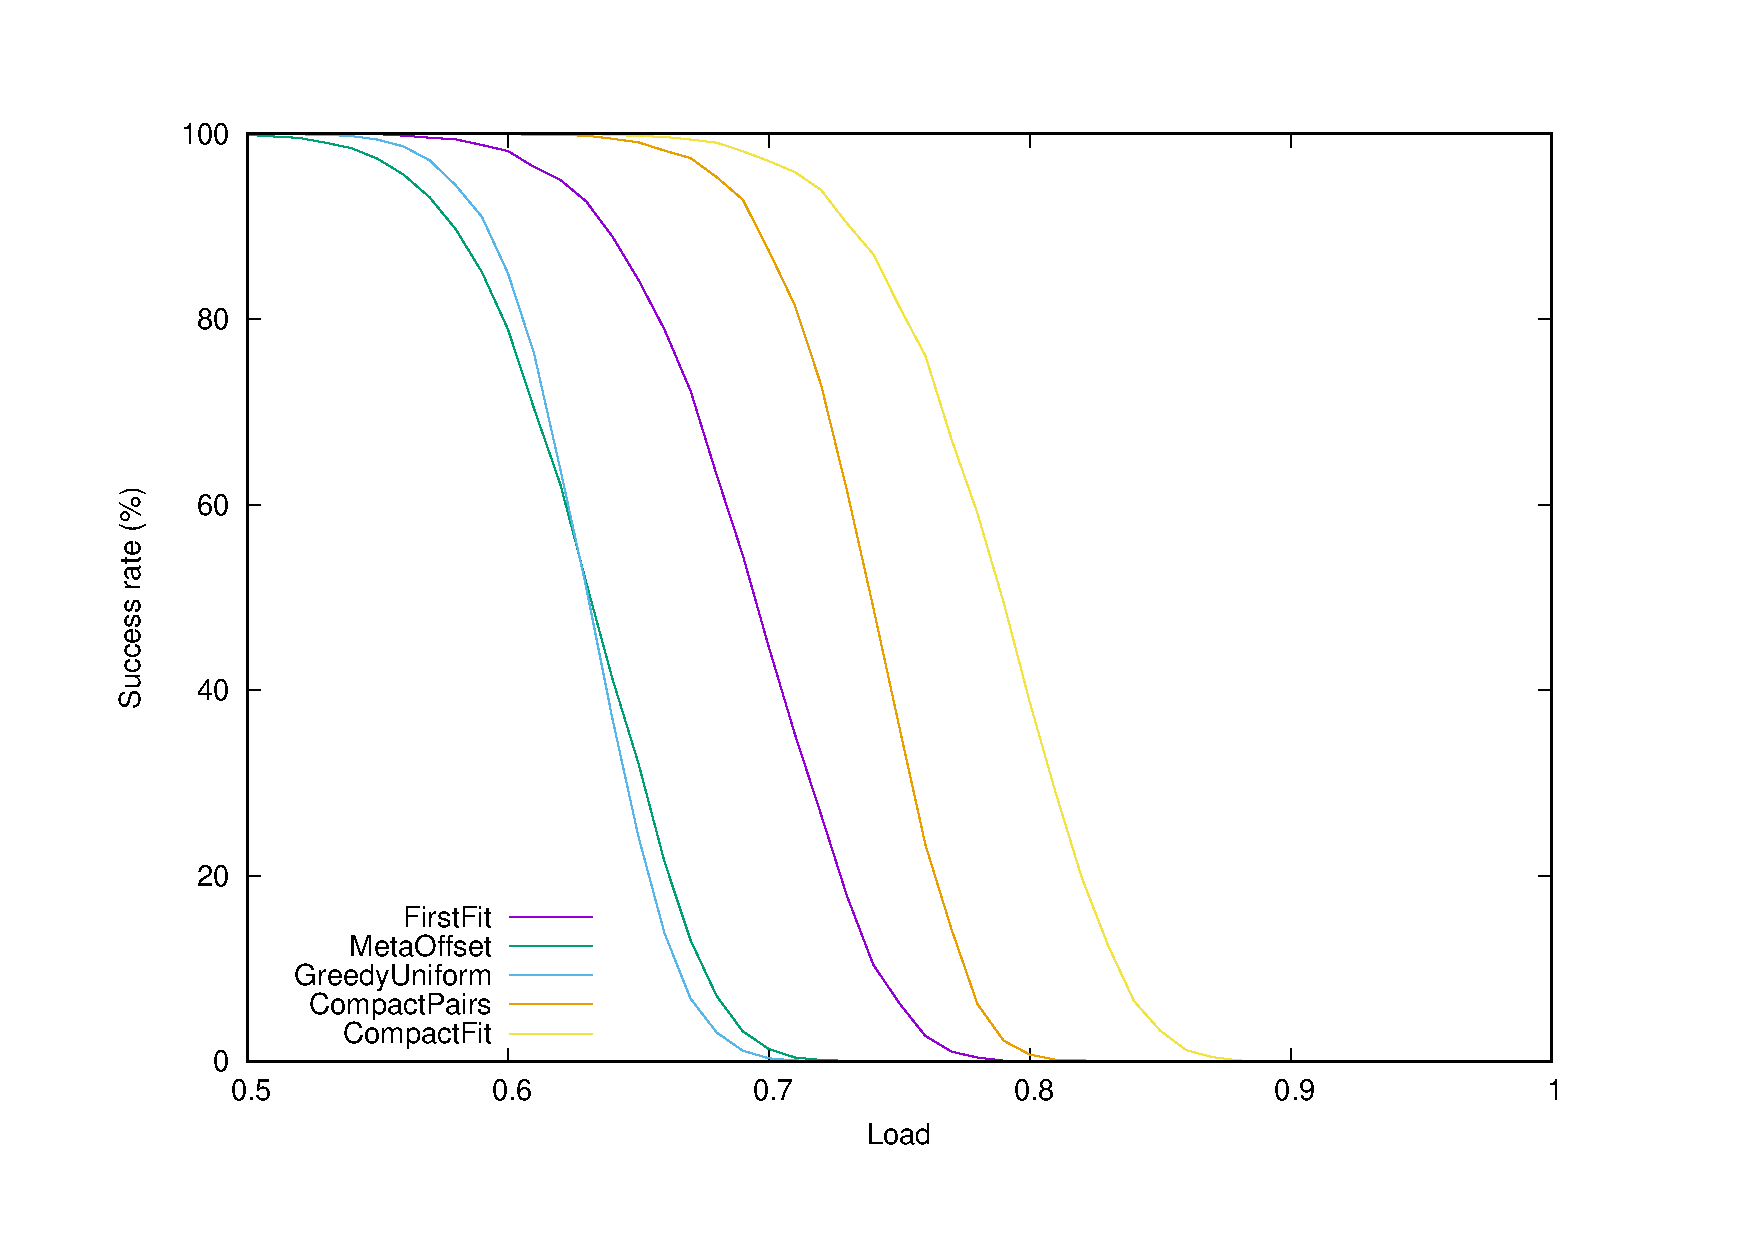
\includegraphics[scale=0.275]{100messBig}

\captionof{figure}{Success rates of all algorithms for increasing loads, $\tau = 1000$, $P=100,000$}
\label{fig:100messBig}
\end{center} 
\end{minipage}
\begin{minipage}[c]{.45\linewidth}
\begin{center}  
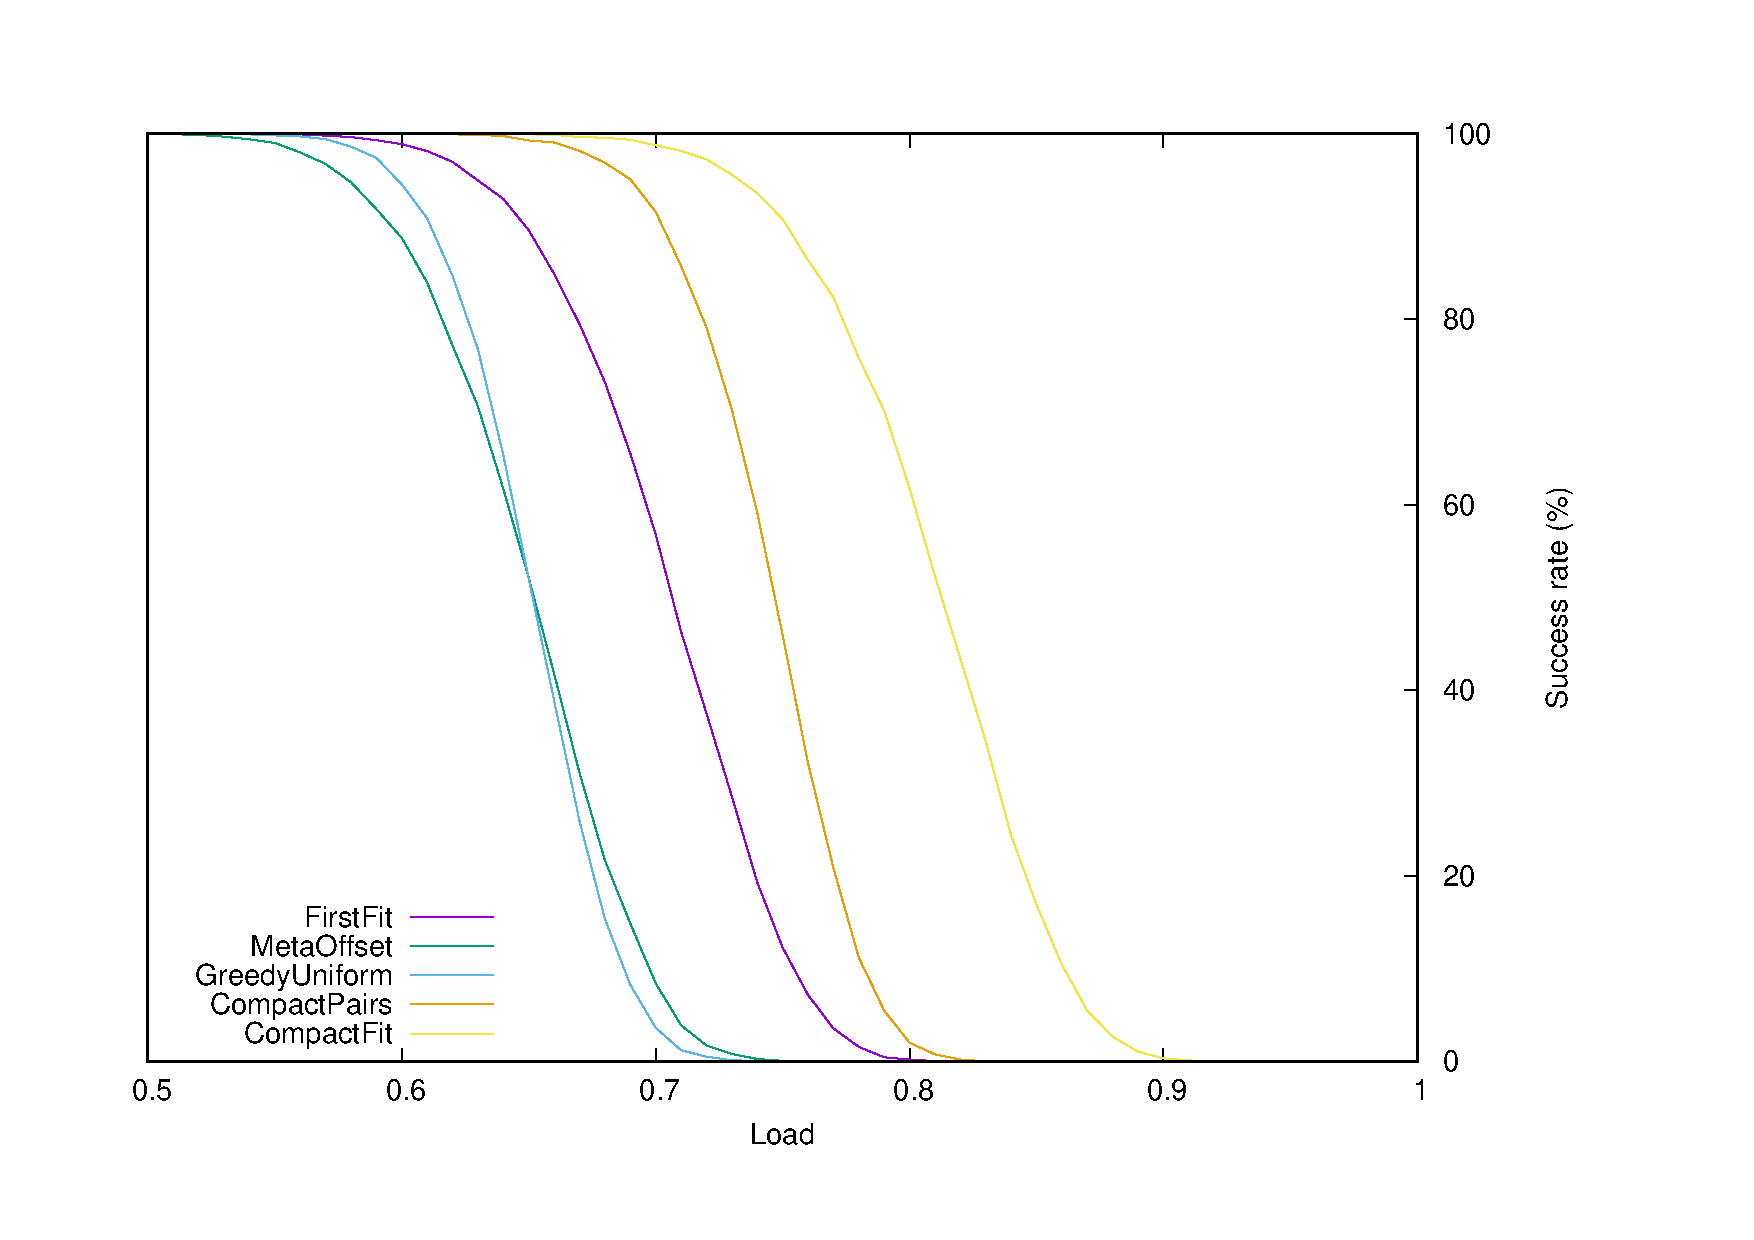
\includegraphics[scale=0.275]{100messSmall}
\captionof{figure}{Success rates of all algorithms for increasing loads, $\tau = 10$, $P=1,000$}
\label{fig:100messSmall}
\end{center}
\end{minipage}



\begin{minipage}[c]{.49\linewidth}

\begin{center}
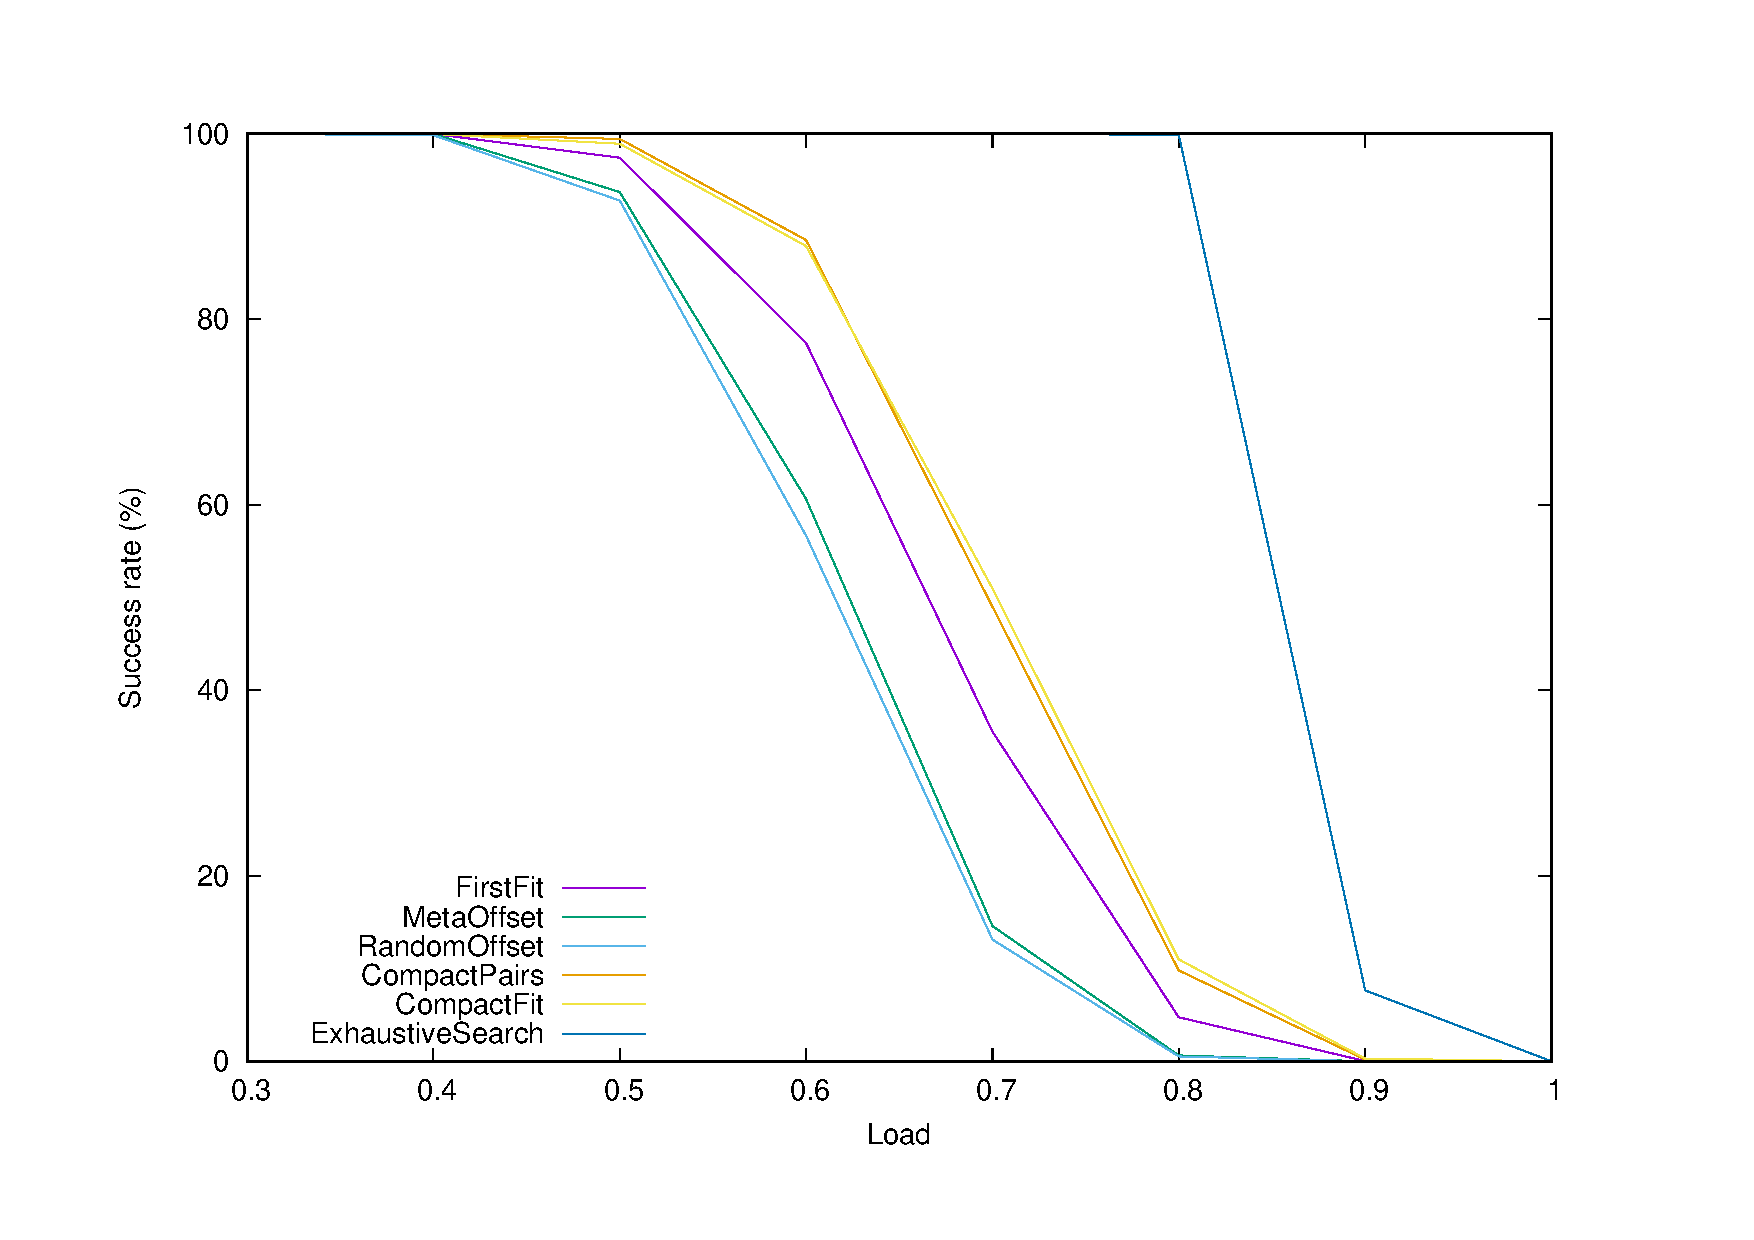
\includegraphics[scale=0.275]{10mess}
\end{center}
\captionof{figure}{Success rates of all algorithms for increasing loads, $\tau = 1000$, $P=10,000$}
\label{fig:10mess}
\end{minipage}
\begin{minipage}[c]{.45\linewidth}
\begin{center}
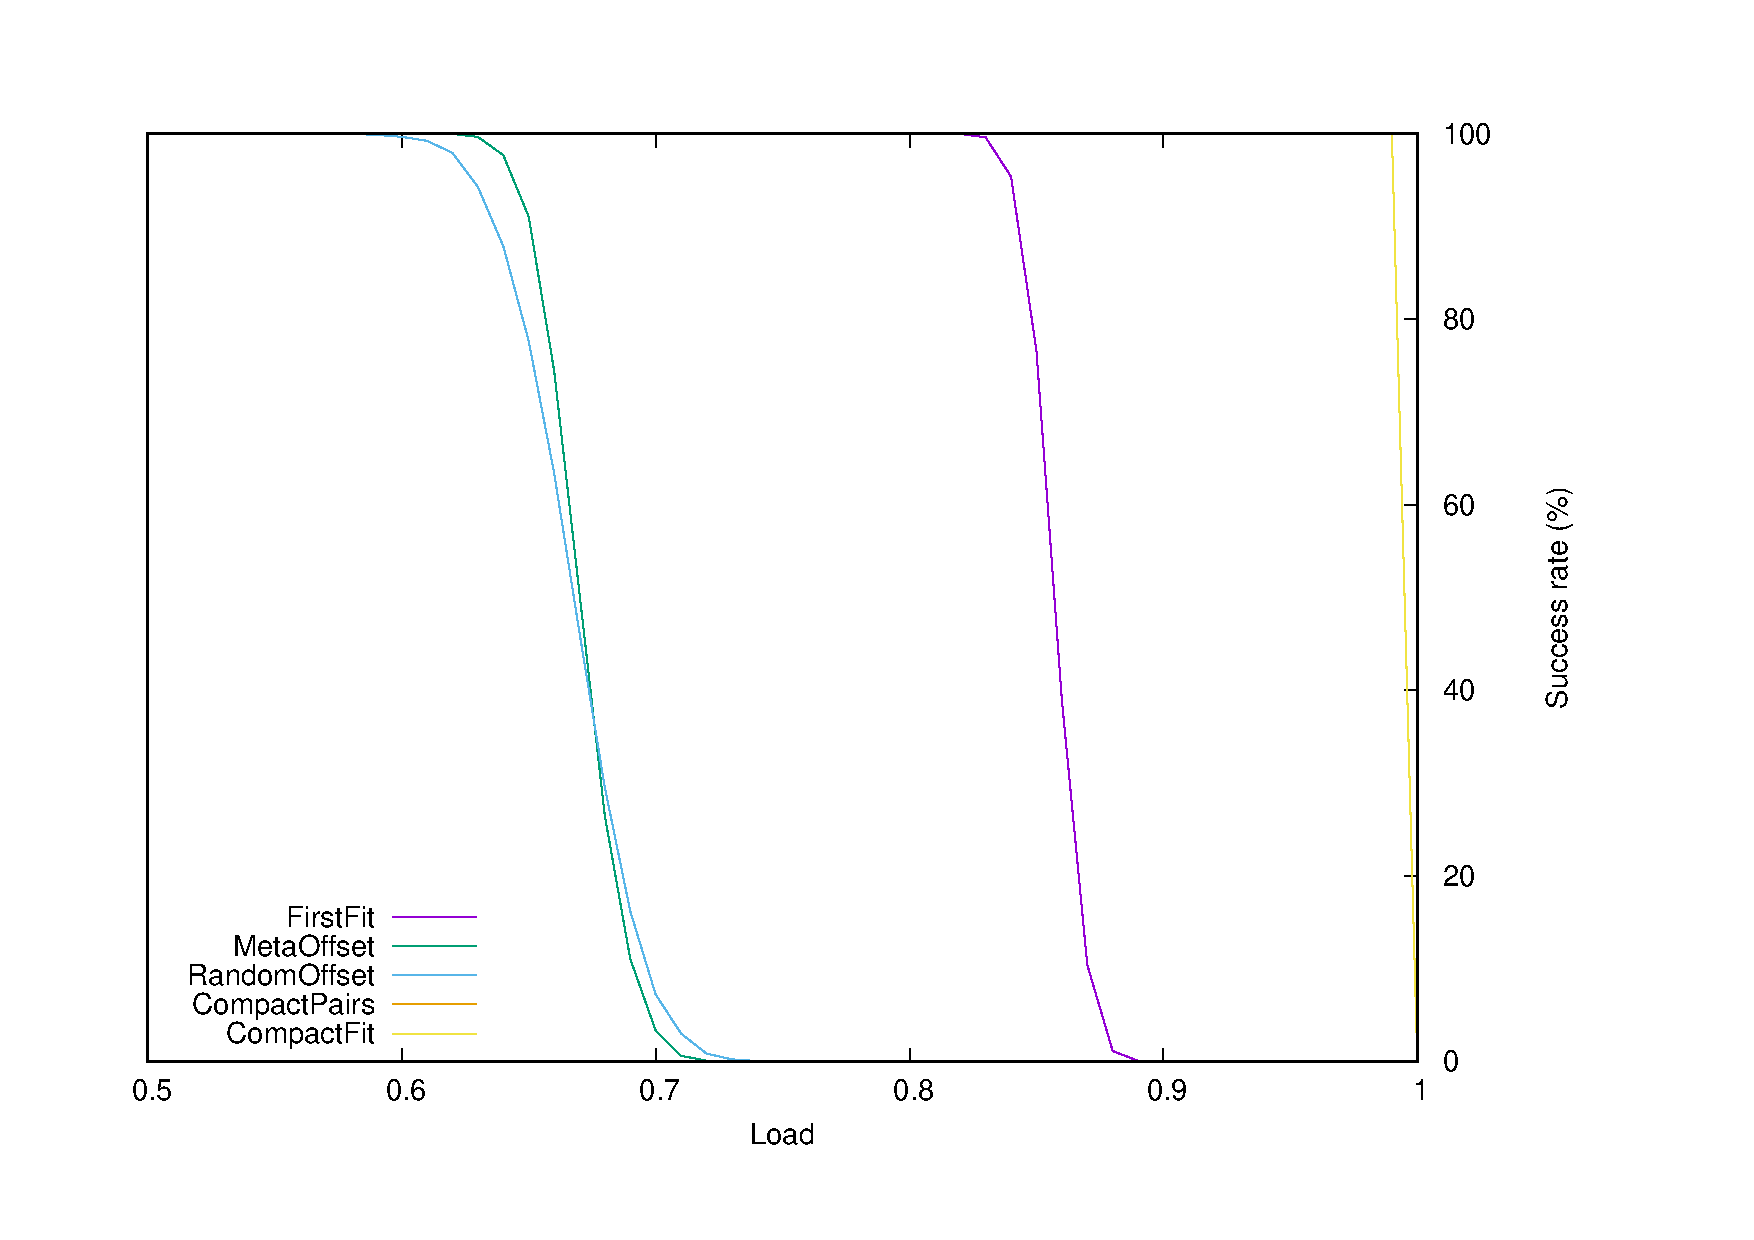
\includegraphics[scale=0.275]{routestau}
\end{center}
\captionof{figure}{Same parameters as in Fig.~\ref{fig:100messBig}, delays uniformly drawn in $[\tau]$}
\label{fig:shortroutes}
\end{minipage}



For all sets of parameters, the algorithms have the same relative performances. \metaoffset and \greedyuniform
perform the worst and have almost equal success rate. Remark that they have a $100\%$ success rate for load
less than $1/2$, while it is easy to build an instance of \pma of load $1/3 +\epsilon$ which makes them fail. 
The difference between the worst case analysis and the average case analysis is explained for \greedyuniform, when $\tau = 1$ in Sec.~\ref{sec:small}.

\firstfit performs better than \metaoffset while they have the same worst case. \compactpair, which is the best theoretically also performs well in the experiments, always finding assignments for load of 
$0.6$.  \compactfit, which is similar in spirit to \compactpair but is designed to have a good success rate on random instances is indeed better than  \compactpair, when there are enough messages.

As demonstrated by Fig.~\ref{fig:100messBig} and Fig.~\ref{fig:100messSmall}, the size of the messages have little impact on the success rate of the algorithms, when the number of messages is constant. Comparing Fig.~\ref{fig:10mess} and Fig.~\ref{fig:100messBig} shows that for more messages, the transition between success rate of $100\%$ to success rate of $0\%$ is faster.
Finally, the results of Exact Resolution in Fig.~\ref{fig:10mess} show that the greedy algorithm are far from always finding a solution when it exists. Moreover, we have found an instance with load $0.8$ with no assignment, which gives an upper bound on the highest load for which \pma can always be solved positively.

We also investigate the behavior of the algorithms when the delay of the messages are drawn in $[\tau]$ in 
Fig.~\ref{fig:shortroutes}. The difference from the case of large delay is that \compactpair and \compactfit are extremely efficent: they always find a solution for $99$ messages. It is expected, since all $d'_i$ are equal in these settings and 
they will both build a $99$-compact tuples and thus can only fail for load $1$.

\subsection{Experimental Results for Small Messages} \label{sec:perf_small}


In this section, the performance on random instances of the algorithms presented in Sec.~\ref{sec:small} is experimentally characterized. The settings are as in Sec.~\ref{sec:perf_large}, with $\tau = 1$. The evaluated algorithms are:

\begin{itemize}
  \item \firstfit
  \item \greedyuniform 
  \item \greedypotential, a greedy algorithm which leverages the notion of potential introduced for Swap. 
  It schedules messages in arbitrary order, choosing the available offset which maximizes the potential of the unscheduled messages
  \item \swapandmove 
  \item \texttt{Exact Resolution}
\end{itemize}

As in Sec.~\ref{sec:perf_large}, the success rate on random instances is much better than the bound given by worst case analysis. In the experiment presented in Fig.~\ref{fig:tau1}, all algorithms succeed on all instances when the load is less than $0.64$. \greedyuniform behaves exactly as proved in Th.~\ref{theorem:uniform}, with a very small variance. The performance of \swapandmove and of its simpler variant \greedypotential, which optimizes the potential in a greedy way, are much better than \firstfit or \greedyuniform. Amazingly, \swapandmove always finds an assignment when the load is less than $0.95$. \swapandmove is extremely close to Exact Resolution, but for $P=10$ and load $0.9$ or $1$, it fails to find some assignments, as shown in Fig.~\ref{fig:tau1-10mess}.

\begin{minipage}[c]{.49\linewidth} 
\begin{center} 
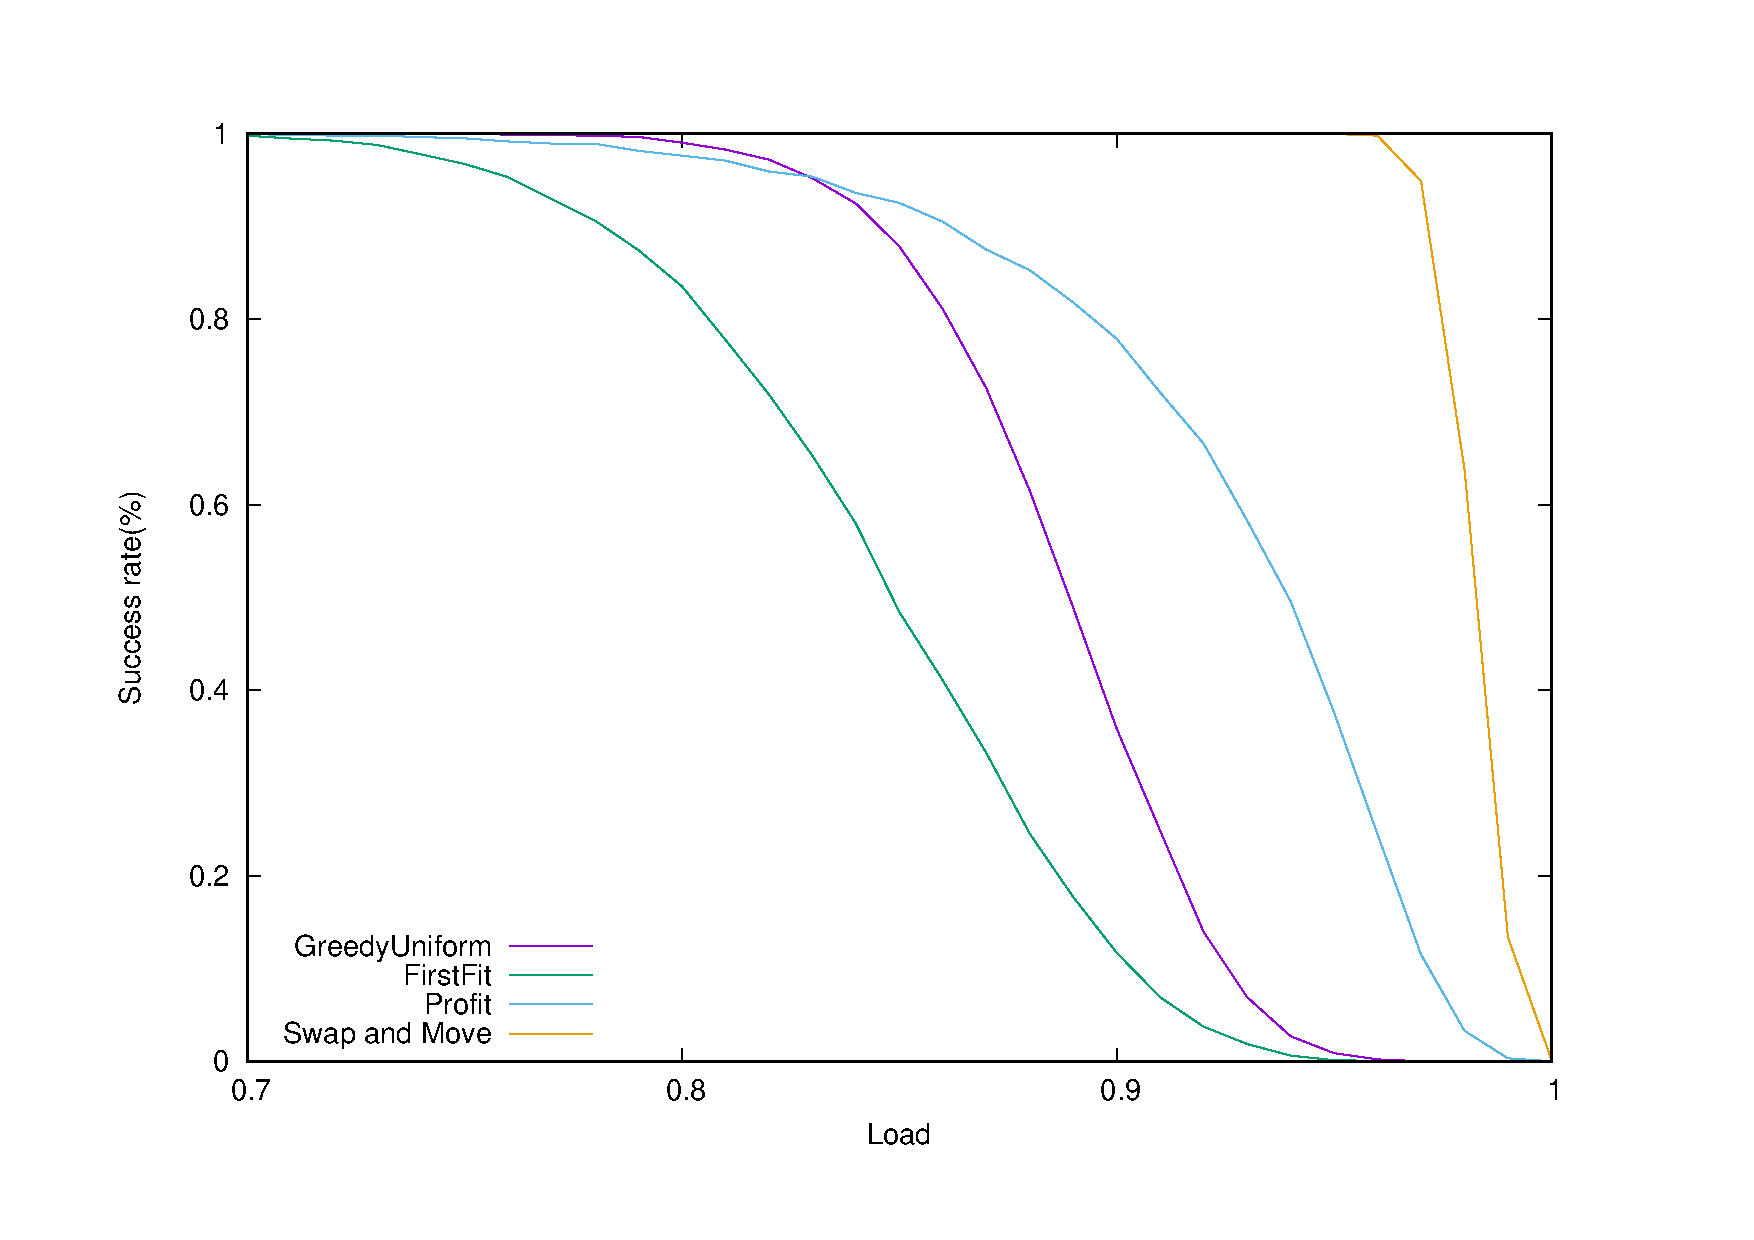
\includegraphics[scale=0.275]{success_tau1} 
\end{center}
\captionof{figure}{Success rates of all algorithms for increasing loads, $\tau = 1$ and $P=100$}
\label{fig:tau1}
\end{minipage}
\begin{minipage}[c]{.45\linewidth} 

\begin{center}
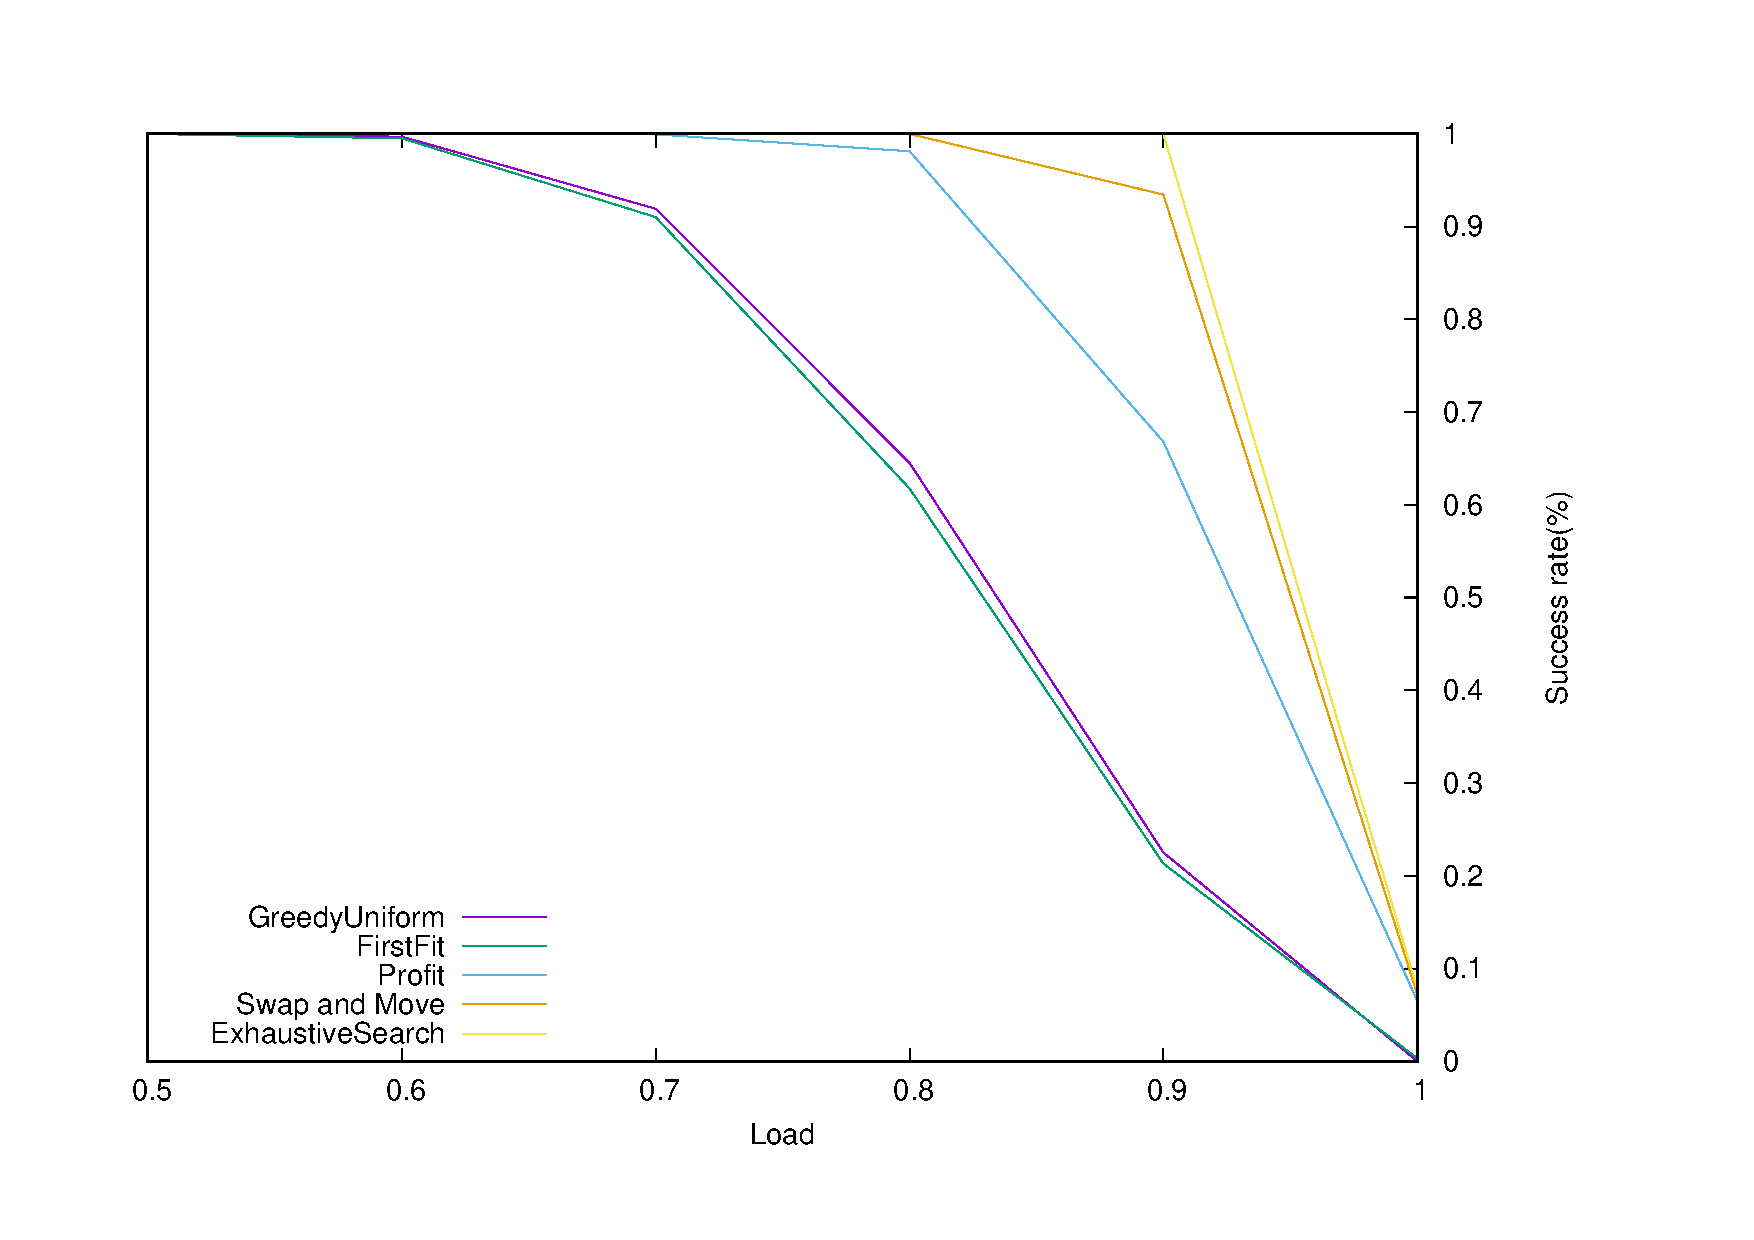
\includegraphics[scale=0.275]{tau110}
\end{center}
\captionof{figure}{Success rates of all algorithms for increasing loads, $\tau = 1$ and $P=10$}
\label{fig:tau1-10mess}
\end{minipage}
 

 Finally, we evaluate the computation times of the algorithms to understand whether they scale to large instances. We present the computation times in Fig.~\ref{fig:timelog} and we choose to consider instances of load $1$, since they require the most computation time for a given size. The empirical complexity of an algorithm is evaluated by a
 linear regression on the function which associates to $\log(n)$, the log of the computation time of the algorithm on $n$ messages.  \firstfit, \greedyuniform and \swapandmove scale almost in the same way, with an empirical complexity slightly below $O(n^2)$, while \greedypotential has an empirical complexity of $O(n^3)$. The empirical complexity corresponds to the worst case complexity we have proved, except for \swapandmove which is in $O(n^3)$ worst case. There are two explanations: most of the messages are scheduled by the fast \firstfit subroutine and most Swap operations improve the potential by more than $1$, as we assume in the worst case analysis.

\begin{figure}
 \begin{center}
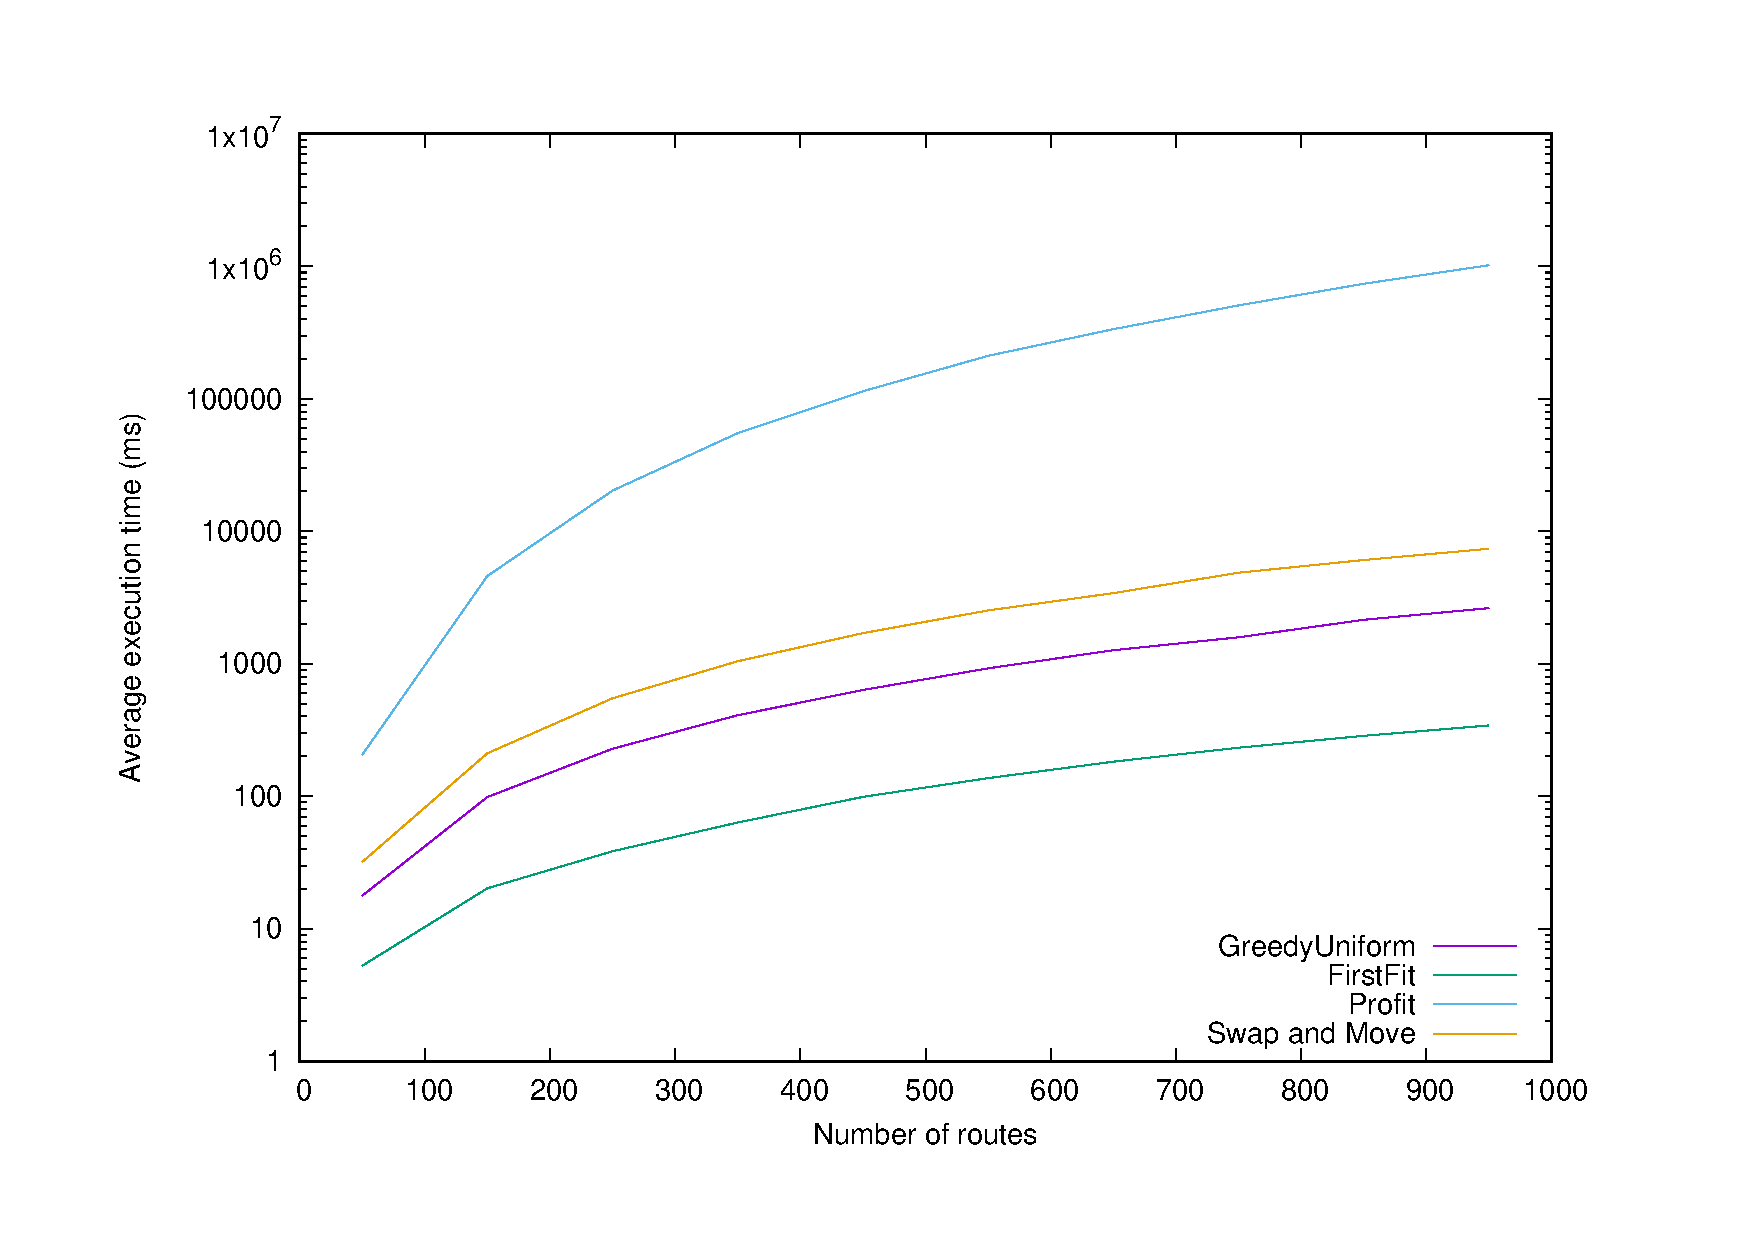
\includegraphics[scale=0.275]{log}
\end{center}
\caption{Computation time (logarithmic scale) function of the number of messages of all algorithms on $10000$ instances of load $1$}
\label{fig:timelog}
\end{figure}

 \bibliography{Sources}

\end{document}
